\providecommand{\toplevelprefix}{../..}  % necessary for subfile bibliography + figures compilation to work, do not move this after documentclass
\documentclass[../../book-main.tex]{subfiles}

\begin{document}

\chapter{Optimization Methods}
\label{app:optimization}

\begin{quote}
``{\em Since the building of all the universe is perfect and is created by the wisdom creator, nothing arises in the universe in which one cannot see the sense of some maximum or minimum.}''

$~$\hfill -- L. Euler
 \end{quote}
\vspace{5mm}

In this chapter, we give a brief introduction to some of the most basic but important optimization algorithms used in this book. The purpose is only to help the reader apply these algorithms to problems studied in this book, not to gain a deep understanding about these algorithms. Hence, we will not provide a thorough justification for the algorithms introduced, in terms of  performance guarantees. 

\section{Steepest Descent}

% {\color{red} TODO ideas for writing this section:
% \begin{enumerate}
%     \item Cover gradient descent from the Taylor expansion perspective. If we want, we can work in nonsmoothness here (Taylor expand the smooth part).
%     Second order info can lead us to write Adam.
%     \item Present some material on diffusion processes for optimizing functions: classical asymptotic convergence results, connections to some modern optimization workflows (how to set batch size, eg).
% \end{enumerate}}

Optimization is concerned with the question of how to find where a function, say $L(\theta)$, reaches its minimum value. Mathematically, this is stated as a problem:
\begin{equation}
    \argmin_{\theta \in \Theta} \cL(\theta),
\end{equation}
where $\Theta$ represents a domain to which the argument $\x$ is confined. Often (and unleess otherwise mentioned, in this chapter) $\Theta$ is simply $\R^n$. Without loss of generality, we assume that here the function $\cL(\theta)$ is smooth\footnote{In case the function \(\cL\) is not smooth, we replace its gradient with a so-called \textit{subgradient}.}. 

The efficiency of finding the (global) minima depends on what information we have about the function \(\cL\). For most optimization problems considered in this book, the dimension of \(\theta\), say \(n\), is very large. That makes computing or accessing local information about \(\ell\) expensive. In particular, since the gradient \(\nabla \cL\) has \(n\) entries, it is often reasonable to compute; however, the Hessian \(\nabla^{2} \cL\) has \(n^{2}\) entries which is often wildly impractical to compute (and the same goes for higher-order derivatives). Hence, it is typical to assume that we have the zeroth-order information, i.e., we are able to evaluate \(\cL(\theta)\), and the first-order information, i.e., we are able to evaluate \(\nabla \cL(\theta)\). Optimization theorists may rephrase this as saying we have a ``first-order \textit{oracle}.'' All optimization algorithms that we introduce in this section only use a first-order oracle.\footnote{We refer the readers to the book by \cite{Wright-Ma-2022} for a more systematic introduction to optimization algorithms in a high-dimensional space, including algorithms assuming higher-order oracles.}  

\subsection{Vanilla Gradient Descent for Smooth Problems}

The simplest and most widely used method for optimization is \textit{gradient descent} (GD). It was first introduced by Cauchy in 1847. The idea is very simple: starting from an initial state, we iteratively take small steps such that each step reduces the value of the function $\cL(\theta)$. 

Suppose that the current state is $\theta$. We want to take a small step, say of distance $h$, in a direction, indicated by a vector $\vv$, to reach a new state $\theta + h\vv$ such that the value of the function decreases:
\begin{equation}
    \cL(\theta + h\vv) \leq \cL(\theta).
\end{equation}
To find such a direction $\vv$, we can approximate $\cL(\theta + h\vv)$ through a Taylor expansion around \(h = 0\):
\begin{equation}
    \cL(\theta + h\vv) = \cL(\theta) + h\ip{\nabla \cL(\theta)}{\vv} + o(h),
\end{equation}
where the inner product here (and in this chapter) will be the \(\ell^{2}\) inner product, i.e., \(\ip{\vx}{\vy} = \vx^{\top}\vy\). To find the direction of \textit{steepest descent}, we attempt to minimize this Taylor expansion among unit vectors \(\vv\). If \(\nabla \cL(\theta) = \vzero\), then the second term above is \(0\) regardless of the value of \(\vv\), so we cannot attempt to make progress, i.e., the algorithm has converged. On the other hand, if \(\nabla \cL(\theta) \neq \vzero\) then it holds 
\begin{equation}\label{eq:steepest_descent_l2_norm}
    \argmin_{\substack{\vv \in \R^{d} \\ \norm{\vv}_{2} = 1}} [\cL(\theta) + h\ip{\nabla \cL(\theta)}{\vv}] = \argmin_{\substack{\vv \in \R^{d} \\ \norm{\vv}_{2} = 1}} \ip{\nabla \cL(\theta)}{\vv} = -\frac{\nabla \cL(\theta)}{\norm{\nabla \cL(\theta)}_{2}},
\end{equation}
In words, this means that the value of \(\cL(\theta + h\vv)\) decreases the fastest along the direction \(\vv = -\nabla \cL(\theta) / \norm{\nabla \cL(\theta)}_{2}\), for small enough \(h\). This leads to the gradient descent method: From the current state $\theta_k$ ($k=0, 1, \ldots$), we take a step of size $h$ in the direction of the negative gradient to reach the next iterate,
\begin{equation}
    \theta_{k+1} = \theta_k - h \nabla \cL(\theta_k). 
\end{equation}
The step size \(h\) is also called the \textit{learning rate} in machine learning contexts.

\subsubsection{Step-Size Selection}

The remaining question is what the step size $h$ should be? If we choose $h$ to be too small, the value of the function may decrease very slowly, as shown by the plot in the middle in \Cref{fig:step-size}. If $h$ is too large, the value might not even decrease at all, as shown by the plot on the right in \Cref{fig:step-size}.

\begin{figure}[h]
    \centering
    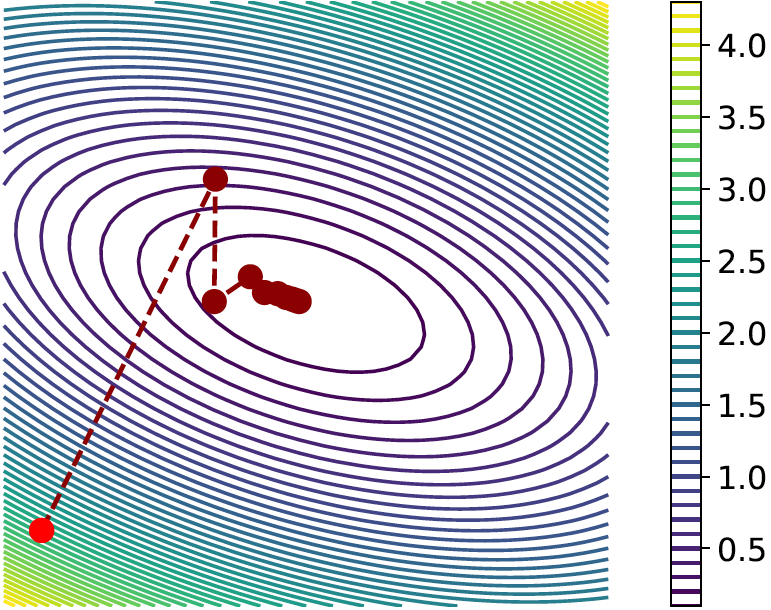
\includegraphics[height=3.5cm]{\toplevelprefix/chapters/appendixA/figs/GD-1.png}
    \hspace{3mm}
    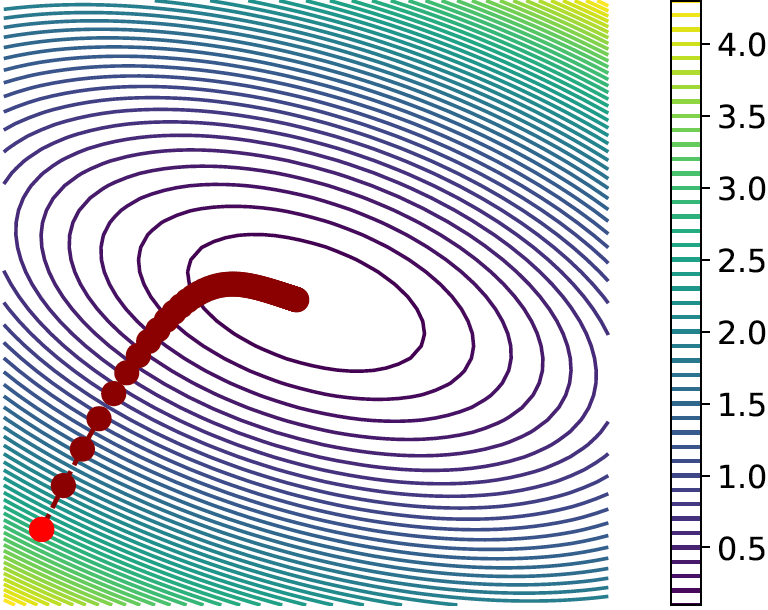
\includegraphics[height=3.5cm]{\toplevelprefix/chapters/appendixA/figs/GD-2.png}
    \hspace{3mm}
    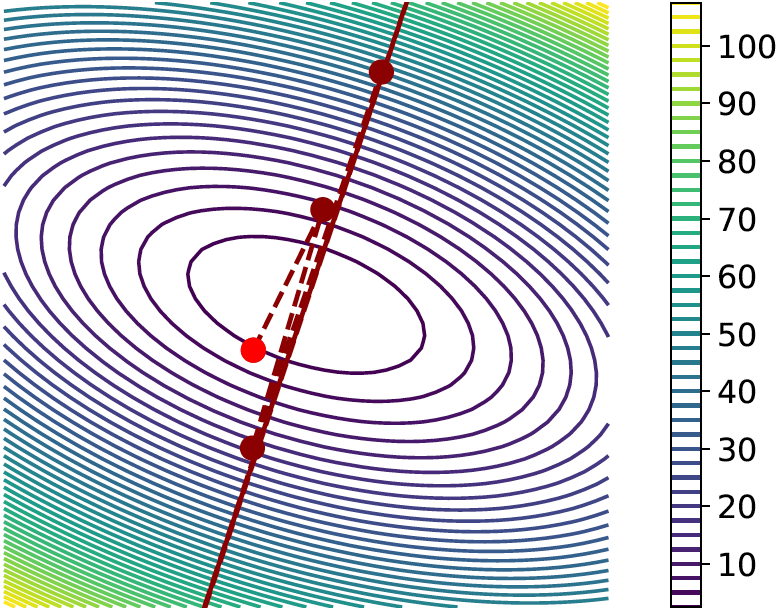
\includegraphics[height=3.5cm]{\toplevelprefix/chapters/appendixA/figs/GD-3.png}
    \caption{The effect of step size $h$ on the convergence of the gradient descent method.}
    \label{fig:step-size}
\end{figure}

So the step size $h$ should be chosen based on the landscape of the function $\cL(\theta_k)$. Ideally, to choose the best step size $h$, we can solve the following optimization problem over a single variable $h$:
\begin{equation}
    h = \argmin_{h\geq 0} \cL(\theta_k - h\nabla \cL(\theta_k)).
\end{equation}
This method of choosing the step size is called \textit{line search}. However, when the function $L(\theta_k)$ is complicated, which is usually the case for training a deep neural network, this one-dimensional optimization is very difficult to solve at each iteration of gradient descent. 

Then how should we choose a proper step size $h$? One common and classical approach is to try to obtain a good approximation of the local landscape around the current state $\theta$ based on some knowledge about the overall landscape of the function $\cL(\theta)$. 

\begin{figure}
    \centering 
    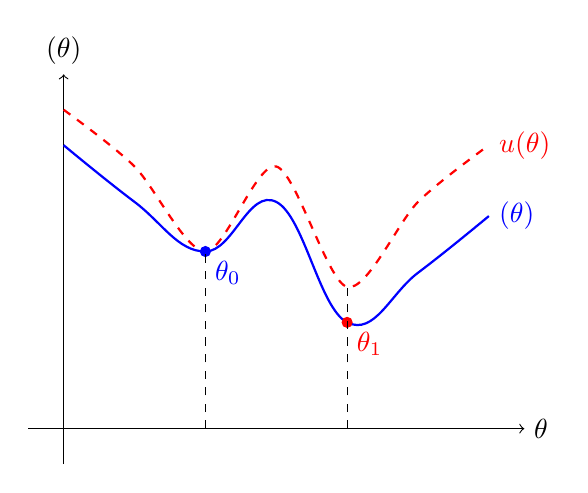
\begin{tikzpicture}[scale=0.9]
        % Axes
        \draw[->] (-0.5,0) -- (6.5,0) node[right] {$\theta$};
        \draw[->] (0,-0.5) -- (0,5) node[above] {$\cL(\theta)$};
        
        % Original function (nonconvex)
        \draw[thick, blue] plot[smooth, tension=0.7] coordinates {
            (0,4) (1,3.2) (2,2.5) (3,3.2) (4,1.5) (5,2.2) (6,3)
        } node[right] {$\cL(\theta)$};
        
        % Upper bound function
        \draw[thick, red, dashed] plot[smooth, tension=0.5] coordinates {
            (0,4.5) (1,3.7) (2,2.5) (3,3.7) (4,2) (5,3.2) (6,4)
        } node[right] {$u(\theta)$};
        
        % Point of equality
        \filldraw[blue] (2,2.5) circle (2pt) node[below right] {$\theta_0$};
        
        % Minimum of upper bound
        \filldraw[red] (4,1.5) circle (2pt) node[below right] {$\theta_1$};
        
        % Vertical lines showing the improvement
        \draw[dashed] (2,0) -- (2,2.5);
        \draw[dashed] (4,0) -- (4,2);
    \end{tikzpicture}
    \caption{\small\textbf{Majorization-minimization scheme and intuition.} A function \(\cL \colon \Theta \to \R\) has a global upper bound \(u \colon \Theta \to \R\) which meets \(L\) at at least one point \(\theta_{0}\). Then, finding the \(\theta_{1}\) which minimizes \(u\) will improve the value of \(\cL\) from \(\cL(\theta_{0})\). Note that similar results can be shown about local upper bounds.}
    \label{fig:majorization_minimization}
\end{figure}

Common conditions for the landscape of \(\cL(\theta)\) include:
\begin{itemize}
    \item \(\alpha\)-Strong Convexity. Recall that \(\cL\) is \textit{\(\alpha\)-strongly convex} if its graph lies above a global quadratic lower bound of slope \(\alpha\), i.e.,
    \begin{equation}
        \cL(\theta) \geq l_{\theta_{0}, \alpha}(\theta) \doteq \cL(\theta_{0}) + \ip{\nabla \cL(\theta_{0})}{\theta - \theta_{0}} + \frac{\alpha}{2}\norm{\theta - \theta_{0}}_{2}^{2}
    \end{equation}
    for any ``base point'' \(\theta_{0}\). We say that \(\cL\) is \textit{convex} if it is \(0\)-strongly convex, i.e., its graph lies above its tangents. It is easy to show (proof as exercise) that strongly convex functions have unique global minima. Another important fact (proof as exercise) is that \(\alpha\)-strongly convex twice-differentiable functions \(\cL\) have (symmetric) Hessians \(\nabla^{2}\cL\) whose minimum eigenvalue is \(\geq \alpha\). For \(\alpha > 0\) this implies the Hessian is symmetric positive definite, and for \(\alpha = 0\) (i.e., \(\cL\) is convex) this implies that the Hessian is symmetric positive semidefinite.
    \item \(\beta\)-Lipschitz Gradient (also called \(\beta\)-Smoothness). Recall that \(\cL\) has \textit{\(\beta\)-Lipschitz gradient} if \(\nabla \cL\) exists and is \(\beta\)-Lipschitz, i.e.,
    \begin{equation}
        \norm{\nabla \cL(\theta) - \nabla \cL(\theta_{0})}_{2} \leq \beta \norm{\theta - \theta_{0}}_{2}.
    \end{equation}
    for any ``base point'' \(\theta_{0}\).  It is easy to show (proof as exercise) that this is equivalent to \(\cL\) having a global quadratic upper bound of slope \(\beta\), i.e.,
    \begin{equation}
        \cL(\theta) \leq u_{\theta_{0}, \beta}(\theta) \doteq \cL(\theta_{0}) + \ip{\nabla \cL(\theta_{0})}{\theta - \theta_{0}} + \frac{\beta}{2}\norm{\theta - \theta_{0}}_{2}^{2}.
    \end{equation}
    for any ``base point'' \(\theta_{0}\).  Another important fact (proof as exercise) is that convex \(\beta\)-Lipschitz gradient twice-differentiable functions have (symmetric) Hessians \(\nabla^{2}\cL\) whose largest eigenvalue is \(\leq \beta\).
\end{itemize}
First, let us suppose that \(\cL\) has \(\beta\)-Lipschitz gradient (but is not necessarily even convex). We will use this occasion to introduce a common optimization theme: \textit{to minimize \(\cL\), we can minimize an upper bound on \(L\)}, which is justified by the following lemma visualized in \Cref{fig:majorization_minimization}.
\begin{lemma}[Majorization-Minimization]\label{lem:majorization_minimization}
    Suppose that \(u \colon \Theta \to \R\) is a global upper bound on \(\cL\), namely \(\cL(\theta) \leq u(\theta)\) for all \(\theta \in \Theta\). Suppose that they meet with equality at \(\theta_{0}\), i.e., \(\cL(\theta_{0}) = u(\theta_{0})\). Then
    \begin{equation}
        \theta_{1} \in \argmin_{\theta \in \Theta}u(\theta) \implies \cL(\theta_{1}) \leq u(\theta_{1}) \leq u(\theta_{0}) = \cL(\theta_{0}).
    \end{equation}
\end{lemma}

We will use this lemma to show that we can use the Lipschitz gradient property to ensure that each gradient step cannot worsen the value of \(\cL\). Indeed, at every base point \(\theta_{0}\), we have that \(u_{\theta_{0}, \beta}\) is a global upper bound on \(\cL\), and \(u_{\theta_{0}, \beta}(\theta_{0}) = \cL(\theta_{0})\). Hence by \Cref{lem:majorization_minimization}
\begin{equation}
    \text{if \(\theta\) minimizes \(u_{\theta_{0}, \beta}\) then} \quad \cL(\theta) \leq u_{\theta_{0}, \beta}(\theta) \leq u_{\theta_{0}, \beta}(\theta_{0}) = \cL(\theta_{0}).
\end{equation}
This motivates us, when finding an update to obtain \(\theta_{k + 1}\) from \(\theta_{k}\), we can instead minimize the upper bound \(u_{\theta_{k}, \beta}\) over \(\theta\) and set that to be \(\theta_{k + 1}\). By minimizing \(u_{\theta_{k}, \beta}\) (proof as exercise) we get 
\begin{equation}\label{eq:GD}
    \theta_{k + 1} = \theta_{k} - \frac{1}{\beta}\nabla \cL(\theta_{k}) \implies \cL(\theta_{k + 1}) \leq \cL(\theta_{k}).
\end{equation}
This implies that a step size \(h = 1/\beta\) is a usable learning rate, but it does not provide a convergence rate or certify that \(L(\theta_{k})\) actually converges to \(\min_{\theta}\cL(\theta)\). This requires a little more rigor, which we now pursue.

Now, let us suppose that \(\cL\) is \(\alpha\)-strongly convex, has \(\beta\)-Lipschitz gradient, and has global optimum \(\theta^{\star}\). We will show that \(\theta_{k}\) will converge directly to the unique global optimum \(\theta^{\star}\), which is a very strong form of convergence. In particular, we will bound \(\norm{\theta^{\star} - \theta_{k}}_{2}\) using both strong convexity and Lipschitzness of the gradient of \(\cL\), i.e., taking a look at the neighborhood around \(\theta_{k}\):\footnote{In this proof the \(\beta\)-Lipschitz Gradient invocation step is a little non-trivial. We also leave this step as an exercise, with the hint to plug in \(\theta = \theta_{0} - h\nabla \cL(\theta_{0})\) into the Lipschitz gradient identity.}
\begin{align}
    \norm{\theta^{\star} - \theta_{k + 1}}_{2}^{2}
    &\leq \norm{\theta^{\star} - \theta_{k} + h\nabla \cL(\theta_{k})}_{2}^{2} \\ 
    &= \norm{\theta^{\star} - \theta_{k}}_{2}^{2} + 2h\ip{\nabla \cL(\theta_{k})}{\theta^{\star} - \theta_{k}} + h^{2}\norm{\nabla \cL(\theta_{k})}_{2}^{2} \\ 
    &\leq \norm{\theta^{\star} - \theta_{k}}_{2}^{2} + 2h\bp{\cL(\theta^{\star}) - \cL(\theta_{k}) - \frac{\alpha}{2}\norm{\theta^{\star} - \theta_{k}}_{2}^{2}} + h^{2}\norm{\nabla \cL(\theta_{k})}_{2}^{2} \quad \text{(\(\alpha\)-SC)} \\
    &= \bp{1 - \alpha h}\norm{\theta^{\star} - \theta_{k}}_{2}^{2} + 2h(\cL(\theta^{\star}) - L(\theta_{k})) + h^{2}\norm{\nabla \cL(\theta_{k})}_{2}^{2} \\
    &\leq \bp{1 - \alpha h}\norm{\theta^{\star} - \theta_{k}}_{2}^{2} + 2h(\cL(\theta^{k}) - \cL(\theta^{\star})) + 2h^{2}\beta(\cL(\theta_{k}) - \cL(\theta^{\star})) \quad \text{(\(\beta\)-LG)} \\
    &= \bp{1 - \alpha h}\norm{\theta^{\star} - \theta_{k}}_{2}^{2} - 2h(1 - \beta h)(\cL(\theta_{k}) - \cL(\theta^{\star})).
\end{align}
In order to ensure that the gradient descent iteration makes progress we must pick the step size so that \(1 - \beta h \geq 0\), i.e., \(h \leq 1/\beta\). If such a setting occurs, then
\begin{align}
    \norm{\theta^{\star} - \theta_{k + 1}}_{2}^{2} 
    &\leq (1 - \alpha h)\norm{\theta^{\star} - \theta_{k}}_{2}^{2} \leq (1 - \alpha h)^{2}\norm{\theta^{\star} - \theta_{k - 1}}_{2}^{2} \leq \cdots \\ 
    &\leq (1 - \alpha h)^{k + 1}\norm{\theta^{\star} - \theta_{0}}_{2}^{2}.
\end{align}
In order to minimize the right-hand side, we can set \(h = 1/\beta\), which obtains 
\begin{equation}
    \norm{\theta^{\star} - \theta_{k + 1}}_{2}^{2} \leq (1 - \alpha/\beta)^{k + 1}\norm{\theta^{\star} - \theta_{0}}_{2}^{2},
\end{equation}
showing convergence to global optimum with exponentially decaying error. Notice that here we used a convergence rate to obtain a favorable \textit{step size} of \(h = 1/\beta\). This motif will re-occur in this section.

We end this section with a caveat: learning a global optimum is (usually) impractically hard. Under certain conditions, we can ensure that the gradient descent iterates converge to a \textit{local optimum}. Also, under more relaxed conditions, we can ensure \textit{local} convergence, i.e., that the iterates converge to a (global or local) optimum if the sequence is initialized close enough to the optimum.

% \DP{TODO: Exercise based on convergence proof for PL condition + Lipschitz gradient.}

\begin{exercise}
    According to the above derivation, for a smooth function $f$, gradient descent converges linearly to the global optimum if it is strongly convex. However, in general nonconvex optimization, we do not have convexity, let alone strong convexity. Fortunately, in some cases, $f$ satisfies the so-called $\mu$-Polyak-Lojasiewicz (PL) inequality, i.e., there exists a constant $\mu > 0$ such that for all $\theta$, 
    \begin{align*}
        \frac{1}{2}\|\nabla f(\theta)\|_2^2 \ge \mu\left( f(\theta) - f(\theta^\star) \right),
    \end{align*}
    where $\theta^*$ is a minimizer of $f$. 
    
    Please show that under the PL inequality and the assumption that $f$ is $\beta$-smooth, gradient descent \eqref{eq:GD} converges linearly to  $\theta^*$. 
\end{exercise}

\subsection{Preconditioned Gradient Descent for Badly-Conditioned Problems}

% \DP{I realized after writing this section that the second-order approximation is not needed for any other section (I thought proximal gradient used second-order approximation but it only needs Lipschitz gradient upper bound). However, I think PSGD is very useful in practice. @YM up to you whether to keep this section.}
% \yima{I think this is ok for now.}

\begin{figure}
    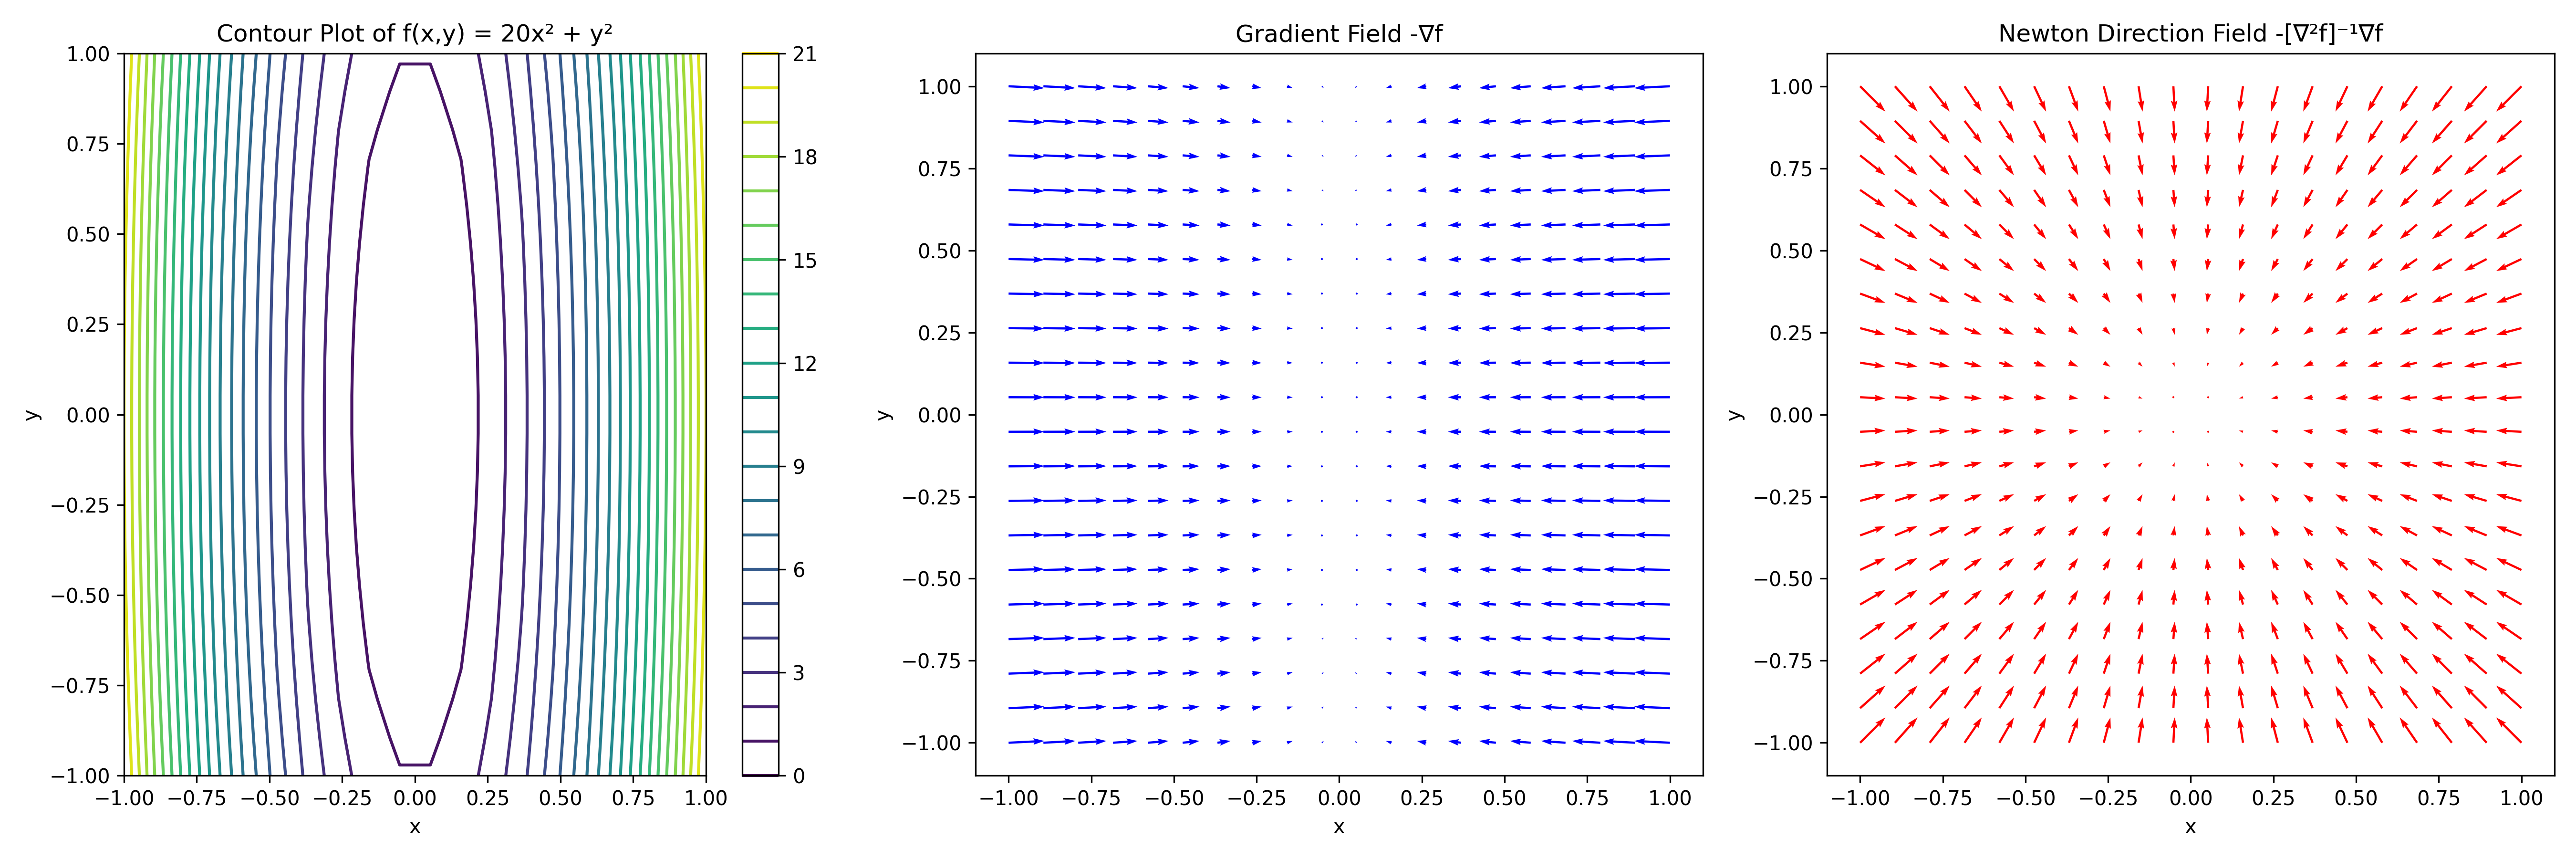
\includegraphics[width=\textwidth]{\toplevelprefix/chapters/appendixA/figs/hessian_geometry.png}
    \caption{\small\textbf{The negative gradient \(-\nabla \cL_{\lambda}\) and pre-conditioned (Newton's method step) vector field \(-[\nabla^{2}\cL_{\lambda}]^{-1}[\nabla \cL_{\lambda}]\)} where \(\lambda = 19\). There is a section of the space where following the negative gradient vector field makes very little progress towards finding the minimum, but in all cases following the Newton's method vector field achieves equal speed of progress towards the optimum since the gradient is whitened. Since the Hessian here is diagonal, adaptive learning rate algorithms (e.g.~Adam, as will be discussed later in the section) can make similar progress as Newton's method, but a non-axis-aligned Hessian may even prevent Adam from succeeding quickly.}
    \label{fig:hessian_geometry}
\end{figure}

\subsubsection{Newton's Method}

There are some smooth problems and strongly convex problems on which gradient descent nonetheless does quite poorly. For example, let \(\lambda \geq 0\) and let \(\cL_{\lambda} \colon \R^{2} \to \R\) of the form 
\begin{equation}
    \cL_{\lambda}(\theta) = \cL_{\lambda}\rp{\mat{\theta_{1} \\ \theta_{2}}} \doteq \frac{1}{2}\bc{(1 + \lambda) \theta_{1}^{2} + \theta_{2}^{2}} = \frac{1}{2}\theta^{\top}\mat{1 + \lambda & 0 \\ 0 & 1}\theta.
\end{equation}
This problem is \(1\)-strongly convex and has \((1 + \lambda)\)-Lipschitz gradient. The convergence rate is then geometric with rate \(1 - 1/(1 + \lambda)\). For large \(\lambda\), this is still not very fast. In this section, we will introduce a class of optimization problems which can successfully optimize such badly-conditioned functions.

The key lies in the objective's \textit{curvature}, which is given by the Hessian. Suppose that (as a counterfactual) we had a \textit{second-order} oracle which would allow us to compute \(\cL(\theta)\), \(\nabla \cL(\theta)\), and \(\nabla^{2}\cL(\theta)\). Then, instead of picking a descent direction \(\vv\) to optimize the first-order Taylor expansion around \(\theta\), we could optimize the second-order Taylor expansion instead. Intuitively this would allow us to incorporate curvature information into the update.

Let us carry out this computation. The second-order Taylor expansion of \(\cL(\theta + h\vv)\) around \(h = 0\) is 
\begin{equation}
    \cL(\theta + h\vv) = \cL(\theta) + h\ip{\nabla \cL(\theta)}{\vv} + \frac{1}{2}h^{2}\ip{[\nabla^{2}\cL(\theta)]\vv}{\vv} + o(h^{2}).
\end{equation}
Then we can compute the descent direction:
\begin{align}
    \argmin_{\substack{\vv \in \R^{n} \\ \norm{\vv}_{2} = 1}}\bs{\cL(\theta) + h\ip{\nabla \cL(\theta)}{\vv} + \frac{1}{2}h^{2}\ip{[\nabla^{2}\cL(\theta)]\vv}{\vv}} 
    &= \argmin_{\substack{\vv \in \R^{n} \\ \norm{\vv}_{2} = 1}}\bs{\ip{\nabla \cL(\theta)}{\vv} + \frac{1}{2}h\ip{[\nabla^{2}\cL(\theta)]\vv}{\vv}}.
\end{align}
This optimization problem is a little difficult to solve because of the constraint \(\norm{\vv}_{2} = 1\). But in practice we never normalize the descent direction \(\vv\) and use the step size \(h\) to control the size of the update. So let us just solve the above problem over all vectors \(\vv \in \R^{n}\):\footnote{If \(\nabla^{2}\cL(\theta)\) is not invertible, then we can replace \([\nabla^{2}\cL(\theta)]^{-1}\) with the Moore-Penrose pseudoinverse of \(\nabla^{2}\cL(\theta)\).}
\begin{equation}
    \argmin_{\vv \in \R^{n}}\bs{\ip{\nabla \cL(\theta)}{\vv} + \frac{1}{2}h\ip{[\nabla^{2}\cL(\theta)]\vv}{\vv}} = -\frac{1}{h}[\nabla^{2}\cL(\theta)]^{-1}[\nabla \cL(\theta)].
\end{equation}
We can thus use the steepest descent iteration 
\begin{equation}
    \theta_{k + 1} = \theta_{k} - [\nabla^{2}\cL(\theta_{k})]^{-1}[\nabla \cL(\theta_{k})],
\end{equation}
(this is the celebrated \textit{Newton's method}), or 
\begin{equation}
    \theta_{k + 1} = \theta_{k} - h[\nabla^{2}\cL(\theta_{k})]^{-1}[\nabla \cL(\theta_{k})],
\end{equation}
(which is called \textit{underdamped Newton's method}). Since the second-order quadratic \(\cL_{\lambda}\) is equal to its second-order Taylor expansion, if we run Newton's method for \textit{one step}, we will achieve the global minimum in \textit{one step} no matter how large \(\lambda\) is. \Cref{fig:hessian_geometry} gives some intuition about poorly conditioned functions and the gradient steps versus Newton's steps.

\subsubsection{PGD}

In practice, we do \textit{not} have a second-order oracle which allows us to compute \(\nabla^{2}\cL(\theta)\). Instead, we can attempt to \textit{learn an approximation to it} alongside the parameter update \(\theta_{k + 1}\) from \(\theta_{k}\). 

How do we learn an approximation to it? We shall find some equations which the Hessian's inverse satisfies and then try to update our approximation so that it satisfies the equations. Namely, taking the Taylor series of \(\nabla \cL(\theta + \delta_{\theta})\) around point \(\theta\), we obtain 
\begin{equation}
    \underbrace{\nabla L(\theta + \delta_{\theta}) - \nabla \cL(\theta)}_{\doteq \delta_{\vg}} = [\nabla^{2} \cL(\theta)]\delta_{\theta} + o(\norm{\delta_{\theta}}_{2}).
\end{equation}
In this case we have 
\begin{equation}
    \delta_{\vg} \approx [\nabla^{2}\cL(\theta)]\delta_{\theta} \implies \delta_{\theta} \approx [\nabla^{2}\cL(\theta)]^{-1}\delta_{\vg}
\end{equation}
We can now try to learn a symmetric positive semidefinite pre-conditioner \(P \in \R^{n \times n}\) such that 
\begin{equation}
    \delta_{\theta} \approx P\delta_{\vg},
\end{equation}
updating it at each iteration along with \(\theta_{k}\). Namely, we have the \textit{PSGD} iteration
\begin{align}
    P_{k}
    &= \mathrm{PreconditionerUpdate}(P_{k - 1}; \theta_{k}, \nabla \cL(\theta_{k})) \\ 
    \theta_{k + 1}
    &= \theta_{k} - hP_{k}\nabla \cL(\theta_{k}).
\end{align}
This update has two problems: how can we even use \(P\) (since we already said we cannot store an \(n \times n\) matrix) and how can we \textit{update} \(P\) at each iteration? The answers are very related; we can never materialize \(P\) in computer memory, but we can represent it using a low-rank factorization (or comparable methods such as \textit{Kronecker factorization} which is particularly suited to the form of deep neural networks). Then the preconditioner update step is designed to exploit the structure of the preconditioner representation.

We end this subsection with a caveat: in deep learning, for example, \(\cL\) is not a convex function and so Newton's method (and approximations to it) do not make sense. In this case we look at the geometric intuition of Newton's method on convex functions, say from \Cref{fig:hessian_geometry}: the inverse Hessian \textit{whitens} the gradients. Thus instead of a Hessian-approximating preconditioner, we can adjust the above procedures to learn a more general whitening transformation for the gradient. This is the idea behind the original proposal of PSGD \cite{li2017preconditioned}, which contains more information about how to store and update the preconditioner, and more modern optimizers like Muon \cite{liu2025muon}.


\subsection{Proximal Gradient Descent for Non-Smooth Problems}\label{subsec:pgd}

Even in very toy problems, however, such as LASSO or dictionary learning, the problem is not strongly convex but rather just convex, and the objective is no longer just smooth but rather the sum of a smooth function and a non-smooth regularizer (such as the \(\ell^{1}\) norm). Such problems are solved by \textit{proximal optimization algorithms}, which generalize steepest descent to non-smooth objectives.

Formally, let us say that 
\begin{equation}
    \cL(\theta) \doteq \cS(\theta) + \cR(\theta)
\end{equation}
where \(\cS\) is smooth, say with \(\beta\)-Lipschitz gradient, and \(\cR\) is non-smooth (i.e., rough). The proximal gradient algorithm generalizes the steepest descent algorithm, by using the majorization-minimization framework (i.e., \Cref{lem:majorization_minimization}) with a different global upper bound. Namely, we construct such an upper bound by asking: what if we take the Lipschitz gradient upper bound of \(S\) but \textit{leave \(R\) alone}?  Namely, we have 
\begin{equation}
    \cL(\theta_{1}) = \cS(\theta_{1}) + \cR(\theta_{1}) \leq u_{\theta_{0}, \beta}(\theta_{1}) \doteq \cS(\theta_{0}) + \ip{\nabla \cS(\theta_{0})}{\theta_{1} - \theta_{0}} + \frac{\beta}{2}\norm{\theta_{1} - \theta_{0}}_{2}^{2} + \cR(\theta_{1}).
\end{equation}
Note that (proof as exercise)
\begin{equation}
    \argmin_{\theta_{1}}u_{\theta_{0}, \beta}(\theta_{1}) = \argmin_{\theta_{1}}\bs{\frac{\beta}{2}\norm*{\theta_{1} - \bp{\theta_{0} - \frac{1}{\beta}\nabla \cS(\theta_{0})}}_{2}^{2} + \cR(\theta_{1})}.
\end{equation}
Now if we try to minimize the upper bound \(u_{\theta_{0}, \beta}\), we are picking a \(\theta_{1}\) that:
\begin{itemize}
    \item is close to the gradient update \(\theta_{0} - \frac{1}{\beta}\nabla \cS(\theta_{0})\);
    \item has a small value of the regularizer \(\cR(\theta_{1})\)
\end{itemize}
and trades off these properties according to the smoothness parameter \(\beta\). Accordingly, let us define the proximal operator
\begin{equation}
    \prox_{h, \cR}(\theta) \doteq \argmin_{\theta_{1}}\bs{\frac{1}{2h}\norm{\theta_{1} - \theta}_{2}^{2} + \cR(\theta)}.
\end{equation}
Then, we can define the \textit{proximal gradient descent} iteration which, at each iteration, minimizes the upper bound \(u_{\theta_{k}, h^{-1}}\), i.e.,
\begin{equation}
    \theta_{k + 1} = \prox_{h, \cR}(\theta_{k} - h\nabla \cS(\theta_{k})).
\end{equation}
Convergence proofs are possible when \(h \leq 1/\beta\), but we do not give any in this section.

One remaining question is: how can we compute the proximal operator? At first
glance, it seems like we have traded one intractable minimization problem for
another. Since we have not made any assumption on \(\cR\) so far, the framework
works even when \(\cR\) is a very complex function (such as a neural network
loss), which would require us to solve a neural network training problem in
order to compute a single proximal operator. However, in practice, for simple
regularizers \(\cR\) such as those we use in this manuscript, there exist
proximal operators which are easy to compute or even in closed-form. We give
a few below (the proofs are an exercise).

\begin{example}\label{example:prox-of-characteristic-function}
    Let \(\Gamma \subseteq \Theta\) be a set, and let \(\chi_{\Gamma}\) be the characteristic function on \(\Gamma\), i.e.,
    \begin{equation}
        \chi_{\Gamma}(\theta) \doteq \casework{0, & \text{if}\ \theta \in \Gamma \\ +\infty, & \text{if}\ \theta \notin \Gamma.}
    \end{equation}
    Then the proximal operator of \(\chi_{\Gamma}\) is a projection, i.e.,
    \begin{equation}
        \prox_{h, \chi_{\Gamma}}(\theta) = \argmin_{\theta_{1} \in \Gamma}\frac{1}{2}\norm{\theta_{1} - \theta}_{2}^{2} = \argmin_{\theta_{1} \in \Gamma}\norm{\theta_{1} - \theta}_{2}.
    \end{equation}
\end{example}

\begin{example}\label{example:prox-of-l1}
    The \(\ell^{1}\) norm has a proximal operator which performs soft thresholding:
    \begin{equation}
        S_{h}(\theta) \doteq \prox_{h, \lambda \norm{\cdot}_{1}}(\theta) = \argmin_{\theta_{1}}\bs{\frac{1}{2h}\norm{\theta_{1} - \theta}_{2}^{2} + \lambda\norm{\theta}_{1}}
    \end{equation}
    then \(S_{h}(\theta)\) is defined by 
    \begin{equation}
        S_{h}(\theta)_{i} = \casework{\theta_{i} - h\lambda, & \text{if}\ \theta_{i} \geq h\lambda \\ 0, & \text{if}\ \theta_{i} \in [-h\lambda, h\lambda] \\ \theta_{i} + h\lambda, & \text{if}\ \theta_{i} \leq -h\lambda} = \casework{\max\{\abs{\theta_{i}} - h\lambda, 0\}\sign(\theta_{i}), & \text{if}\ \abs{\theta_{i}} \geq h\lambda \\ 0, & \text{if}\ \abs{\theta_{i}} < h\lambda.}
    \end{equation}
    The proximal gradient operation with the smooth part of the objective being least-squares and the non-smooth part being the \(\ell^{1}\) norm (hence using this soft thresholding proximal operator) is called the Iterative Shrinkage-Thresholding Algorithm (ISTA).
\end{example}

\begin{example}\label{example:prox-of-nonnegative-l1}
    In \Cref{ch:representation} we use a proximal operator corresponding to the \(\ell^{1}\) norm plus the characteristic function for the positive orthant \(\R_{+}^{n} \doteq \{\vx \in \R^{n} \colon x_{i} \geq 0\ \forall i\}\), namely
    \begin{equation}
        T_{h}(\theta) \doteq \prox_{h, \lambda\norm{\cdot}_{1} + \chi_{\R_{+}^{n}}}(\theta) = \argmin_{\theta_{1} \in \R_{+}^{n}}\bs{\frac{1}{2h}\norm{\theta_{1} - \theta}_{2}^{2} + \lambda\norm{\theta}_{1}},
    \end{equation}
    then \(T_{h}\) is defined as 
    \begin{equation}
        T_{h}(\theta)_{i} \doteq \max\{\theta_{i} - h\lambda, 0\}.
    \end{equation}
    This proximal operator yields the non-negative ISTA that is invoked in \Cref{ch:representation} and beyond.
\end{example}


% \DP{Optional: @SB want to put some stuff in about learning a prox}

\subsection{Stochastic Gradient Descent for Large-Scale Problems}

% \yima{Maybe here introducing stochastic gradient descent for the case when $f(\x)$ needs to be estimated as an expectation $f(\x) = \mathbb{E}_{\boldsymbol{w}}(f(\x, \boldsymbol{w})$ samples of another random variable $\boldsymbol{w}$, as in the case of training a neural networks with an expected loss over a batch of samples. Druv or Sam? One problem is that here we use $\x$ as the optimization variable but in the deep networks below we use $\bm(\theta)$... and $\x$ for the samples. Make notation better later!}

In deep learning, the objective function \(\cL\) usually cannot be computed exactly, and instead at each optimization step it is \textit{estimated} using finite samples (say, using a mini-batch). A common way to model this situation is to define a \textit{stochastic loss function} \(\cL_{\omega}(\theta)\) where \(\omega\) is some ``source of randomness''. For example, \(\omega\) could contain the indices of the samples in a batch over which to compute the loss. Then, we would like to minimize \(\cL(\theta) \doteq \Ex_{\omega}[\cL_{\omega}(\theta)]\) over \(\theta\), given access to a \textit{stochastic first-order oracle}: given \(\theta\), we can sample \(\omega\) and compute \(\cL_{\omega}(\theta)\) and \(\nabla_{\theta}\cL_{\omega}(\theta)\). This minimization problem is called a \textit{stochastic optimization problem}.

The basic first-order stochastic algorithm is \textit{stochastic gradient descent}: at each iteration \(k\) we sample \(\omega_{k}\), define \(\cL_{k} \doteq \cL_{\omega_{k}}\), and perform a gradient step on \(\cL_{k}\), i.e.,
\begin{equation}
    \theta_{k + 1} = \theta_{k} - h\nabla \cL_{k}(\theta_{k}).
\end{equation}
However, even for very simple problems we cannot expect the same type of convergence as we obtained in gradient descent. For example, suppose that there are \(m\) possible values for \(\omega \in \{1, \dots, m\}\) which it takes with equal probability, and there are \(m\) possible targets \(\xi_{1}, \dots, \xi_{m}\), such that the loss function \(\cL_{\omega}\) is
\begin{equation}
    \cL_{\omega}(\theta) \doteq \frac{1}{2}\norm{\theta - \xi_{\omega}}_{2}^{2}.
\end{equation}
Then \(\argmin_{\theta}\Ex[\cL_{\omega}(\theta)] = \frac{1}{m}\sum_{i = 1}\xi_{i}\), but stochastic gradient descent can ``pinball'' around the global optimum value, and not converge, as visualized in \Cref{fig:sgd_nonconvergence}. 

\begin{figure}
    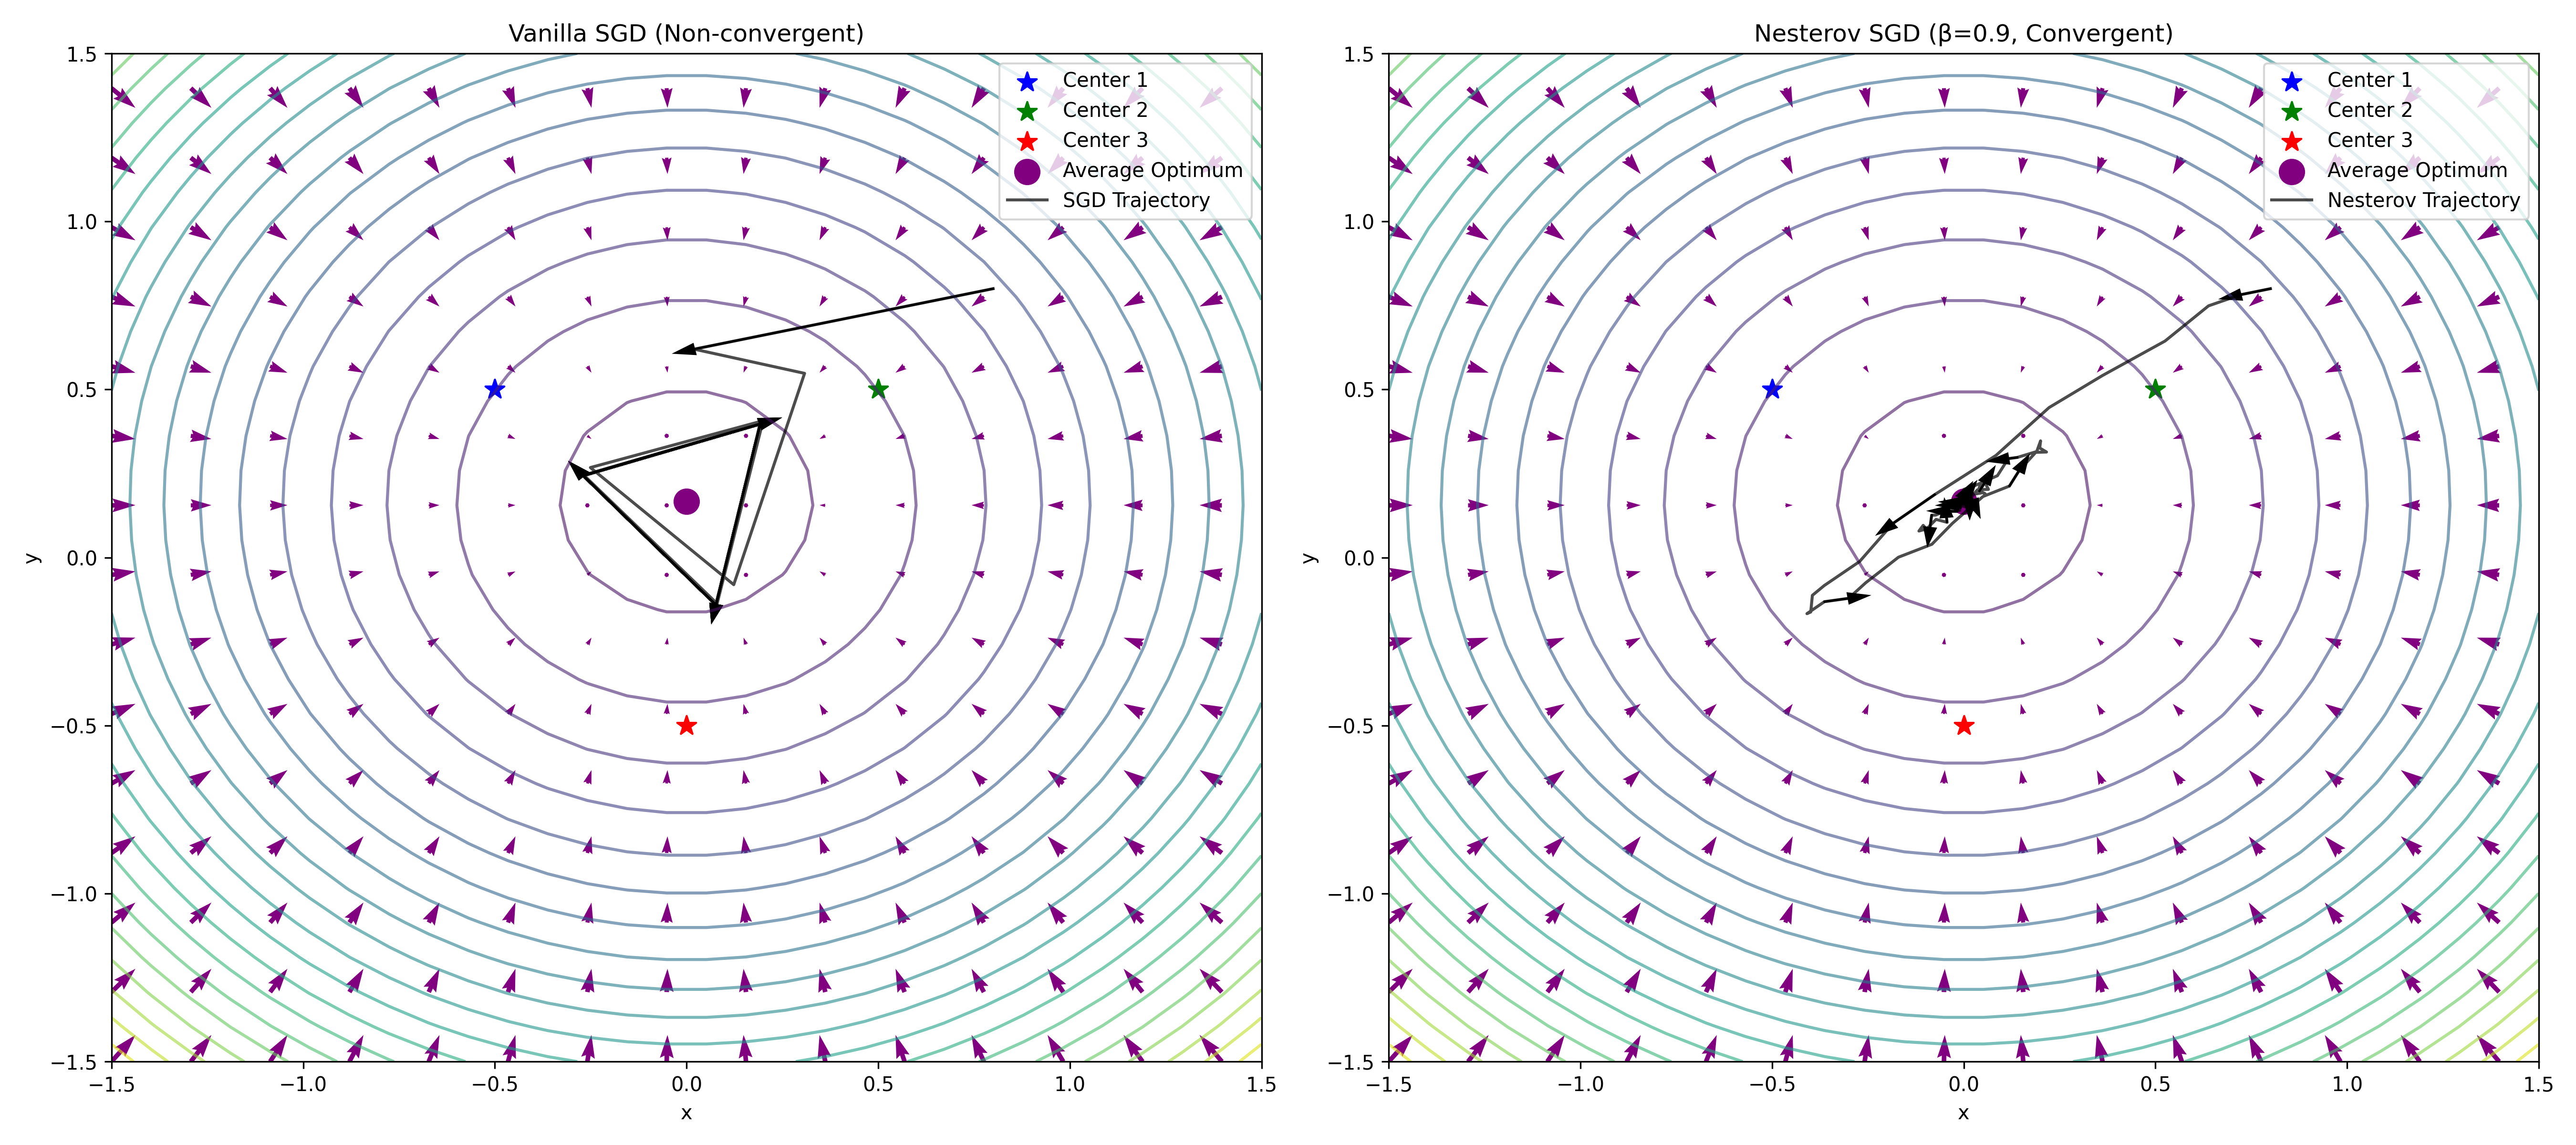
\includegraphics[width=\textwidth]{\toplevelprefix/chapters/appendixA/figs/sgd_vs_nesterov.png}
    \centering 
    \caption{\small\textbf{Stochastic gradient descent may not converge, even for very benign objectives, but Nesterov gradient converges.} For even simple quadratic objectives, stochastic gradient descent iterates may pinball around the global optimum, whereas Nesterov gradients align to point to the optimal value.}
    \label{fig:sgd_nonconvergence}
\end{figure}

In order to fix this, we can either average the parameters \(\theta_{k}\) or average the gradients \(\nabla \cL_{k}(\theta_{k})\) over time. If we average the parameters \(\theta_{k}\), then (using \Cref{fig:sgd_nonconvergence} as a mental model) the issue of pinballing is straightforwardly not possible, since the average iterate will grow closer to the center. As such, most theoretical convergence proofs consider the convergence of the average iterate \(\frac{1}{k}\sum_{i = 0}^{k}\theta_{i}\) to the global minimum. If we average the gradients, we will eventually learn an average gradient \(\frac{1}{k}\sum_{i = 0}^{k}\nabla \cL_{k}(\theta_{k})\) which does not change much at each iteration and therefore does not pinball.

In practice, instead of using an arithmetic average, we take an \textit{exponentially moving average} (EMA) of the parameters (this is called \textit{Polyak momentum}) or of the gradients (this is called \textit{Nesterov momentum}). Nesterov momentum is more popular and we will study it here.

A stochastic gradient descent iteration with Nesterov momentum is as follows:
\begin{align}
    \vg_{k}
    &= \beta\vg_{k - 1} + (1 - \beta)\nabla \cL_{k}(\theta_{k}) \\ 
    \theta_{k + 1}
    &= \theta_{k} - h\vg_{k}.
\end{align}
We do not go through a convergence proof (see Chapter 7 of \cite{garrigos2023handbook} for an example). However, Nesterov momentum handles our toy case in \Cref{fig:sgd_nonconvergence} easily (see the right-hand figure): it stops pinballing and eventually converges to the global optimum.

We end with a caveat: one can show that Polyak momentum and Nesterov momentum are equivalent, for certain choices of parameter settings. Then it is also possible to show that a decaying learning rate schedule (i.e., the learning rate \(h\) depends on the iteration \(k\), and its limit is \(h_{k} \to 0\) as \(k \to \infty\)) with plain SGD (or PSGD) can mimic the effect of momentum. Namely, \cite{defazio2023optimal} shows that if the SGD algorithm lasts \(K\) iterations, the gradient norms are bounded \(\norm{\nabla \cL(\theta_{k})}_{2} \leq G\), and we define \(D \doteq \norm{\theta_{0} - \theta^{\star}}_{2}\), then plain SGD iterates \(\theta_{k}\) satisfy the rate \(\Ex[\cL(\theta_{k}) - \cL(\theta^{\star})] \leq DG/\sqrt{K}\) --- but only so long as the learning rate \(h_{k} = (D/[G\sqrt{K}])(1 - k/K)\) decays \textit{linearly} with time. This matches learning rate schedules used in practice. Indeed, surprisingly, such a theory of convex optimization can predict many empirical phenomena in deep networks \cite{schaipp2025surprising}, despite deep learning optimization being highly non-convex and non-smooth in the worst case. It is so far unclear why this is the case.


\subsection{Putting Everything Together: Adam}

The gradient descent scheme proposes an iteration of the form 
\begin{equation}
    \theta_{k + 1} = \theta_{k} + h\vv_{k},
\end{equation}
where (recall) \(\vv_{k}\) is chosen to be (proportional to) the steepest descent vector in the Euclidean norm:
\begin{equation}
    \vv_{k} = -\frac{\nabla \cL(\theta_{k})}{\norm{\nabla \cL(\theta_{k})}_{2}} \in \argmin_{\substack{\vv \in \R^{n} \\ \norm{\vv}_{2} = 1}}\ip{\nabla \cL(\theta_{k})}{\vv}.
\end{equation}
However, in the context of deep learning optimization, there is absolutely nothing which implies that we have to use the Euclidean norm; indeed the ``natural geometry'' of the space of parameters is not well-respected by the Euclidean norm, since small changes in the parameter space can lead to very large differences in the output space, for a particular fixed input to the network. If we were instead to use a generic norm \(\norm{\cdot}\) on the parameter space \(\R^{n}\), we would get some other quantity corresponding to the so-called \textit{dual norm}:
\begin{equation}
    \vv_{k} \in \argmin_{\substack{\vv \in \R^{n} \\ \norm{\vv} = 1}}\ip{\nabla \cL(\theta_{k})}{\vv}.
\end{equation}
For instance, if we were to use the \(\ell^{\infty}\)-norm, it is possible to show that 
\begin{equation}
    \vv_{k} = -\sign(\nabla \cL(\theta_{k})) \in \argmin_{\substack{\vv \in \R^{n} \\ \norm{\vv}_{\infty} = 1}}\ip{\nabla \cL(\theta_{k})}{\vv},
\end{equation}
where \(\sign(\vx)_{i} = \sign(x_{i}) \in \{-1, 0, 1\}\). Thus if we were so-inclined, we could use the so-called \textit{sign-gradient descent}:
\begin{equation}\label{eq:sign_gradient_descent}
    \theta_{k + 1} = \theta_{k} - h\sign(\nabla \cL(\theta_{k})).
\end{equation}
From sign-gradient descent, we can derive the famous Adam optimization algorithm. Note that for a scalar \(x \in \R\) we can write
\begin{equation}
    \sign(x) = \frac{x}{\abs{x}} = \frac{x}{\sqrt{x^{2}}}.
\end{equation}
Similarly, for a vector \(\vx \in \R^{n}\) we write (where \(\hada\) and
\(\haddiv\) are element-wise multiplication and division)
\begin{equation}
    \sign(\vx) = \vx \haddiv [\vx^{\hada 2}]^{\hada (1/2)}.
\end{equation}
Using this representation we can write \eqref{eq:sign_gradient_descent} as 
\begin{equation}
    \theta_{k + 1} = \theta_{k} - h ([\nabla \cL(\theta_{k})] \haddiv [\nabla
    \cL(\theta_{k})^{\hada 2}]^{\hada \frac{1}{2}}).
\end{equation}
Now consider the stochastic regime where we are optimizing a different loss \(L_{k}\) at each iteration. In SGD, we ``tracked'' (i.e., took an average of) the gradients using Nesterov momentum. Here, we can track both the gradient and the squared gradient using momentum, i.e.,
\begin{align}
    \vg_{k}
    &= \beta^{1}\vg_{k - 1} + (1 - \beta^{1})\nabla \cL_{k}(\theta_{k}) \\ 
    \vs_{k}
    &= \beta^{2}\vs_{k - 1} + (1 - \beta^{2})[\nabla \cL_{k}(\theta_{k})]^{\hada 2}  \\
    \theta_{k + 1}
    &= \theta_{k} - h\vg_{k}\haddiv\vs_{k}^{\hada \frac{1}{2}},
\end{align}
where \(\beta^{i} \in [0, 1]\) are the momentum parameters. The algorithm
presented by this iteration is the celebrated \textit{Adam}
optimizer,\footnote{In order to avoid division-by-zero errors, we divide by
\(\vs_{k}^{\hada (1/2)} + \eps \vone_{n}\) where \(\eps\) is small, say on the order of \(10^{-8}\).} which is the most-used optimizer in deep learning. While convergence proofs of Adam are more involved, it falls out of the same steepest descent principle we used so far, and so we should expect that given a small enough learning rate, each update should improve the loss.

Another way to view Adam, which partially explains its empirical success, is that it dynamically updates the learning rates for each parameter based on the squared gradients. In particular, notice that we can write
\begin{equation}
    \theta_{k + 1} = \theta_{k} - \eta_{k} \hada \vg_{k} \qquad \text{where}
    \qquad \eta_{k} = h \vs_{k}^{\hada (-\frac{1}{2})}
\end{equation}
where \(\eta_{k}\) is the parameter-wise adaptively set learning rate. This scheme is called adaptive because if the gradient of a particular parameter is large up to iteration \(k\), then the learning rate for this parameter becomes smaller to compensate, and vice versa, as can be seen from the above equation.


% \subsection{Theoretical Toolkit: Gradient Flow}

% Let us suppose that the sequence of parameters \(\theta_{k}\) generated by \textit{gradient descent} with step size \(h\) were actually sampled from a differentiable function \(\theta \colon \R \to \R^{n}\), where \(\theta(kh) = \theta_{k}\). What would the laws governing this continuous-time realization look like?

% To explore this, let us write out the gradient descent dynamics
% \begin{equation}
%     \theta_{k + 1} = \theta_{k} - h\nabla \cL(\theta_{k}).
% \end{equation}
% Defining \(\theta(\cdot)\) as above, i.e.,
% \begin{equation}
%     \theta(t) = \theta_{\floor{t/h}}, \qquad \forall t.
% \end{equation}
% It holds that
% \begin{equation}
%     \theta(t + h) = \theta_{\floor{(t + h)/h}} = \theta_{\floor{t/h} + 1} = \theta_{\floor{t/h}} - h\nabla \cL(\theta_{\floor{t/h}}) = \theta(t) - h\nabla \cL(\theta(t)).
% \end{equation}
% Dividing both sides by \(h\) and taking the limit \(h \to 0\), it holds 
% \begin{equation}
%     \dot{\theta}(t) = \lim_{h \to 0}\frac{\theta(t + h) - \theta(t)}{h} = -\cL(\theta(t)),
% \end{equation}
% where \(\dot{\theta}(t) = \odv{\theta}{t}(t)\) is the time-derivative of \(\theta\). The continuous-time dynamics of \(\theta\) are therefore given by the so-called \textit{gradient flow} ODE
% \begin{equation}
%     \dot{\theta}(t) = -\nabla \cL(\theta(t)).
% \end{equation}
% Notice that the continuous-time gradient flow and the discrete-time gradient descent are not necessarily equal to each other for any finite step size \(h\). Nonetheless, for sufficiently small \(h\), it is often possible to show that the approximation error between \(\theta_{\floor{t/h}}\) and \(\theta(t)\) is small.

% Often, theoretical results in the literature are about the gradient flow rather than the gradient descent. There are several reasons for this, aptly summarized in the blog post \cite{bach2020effortless}. The main pro and con are:
% \begin{itemize}
%     \item The analysis of gradient flow is greatly simplified, as we do not need to consider step sizes, and calculus makes proving certain identities much easier compared to bounding finite sums.
%     \item However, the analysis of gradient flow is hard to rigorously transfer to discrete-time gradient descent. Still, gradient flow is usually a good approximation to gradient descent with very small step sizes.
% \end{itemize}
% Notably, it is possible to devise models for Nesterov-momentum GD, Adam, and SGD; the former two are left as exercises, while the latter is out of scope of this book as it requires more sophisticated mathematical modeling than is presented in the book.

% To show why gradient flow is so much nicer to analyze, we show that \(\cL\) decreases along the gradient flow even when it is nonconvex, i.e.,
% \begin{equation}
%     \odv*{\cL(\theta(t))}{t} = \ip{\dot{\theta}(t)}{\nabla_{\theta}\cL(\theta(t))} = -\norm{\nabla_{\theta}\cL(\theta(t))}_{2}^{2} \leq 0.
% \end{equation}
% Therefore, running gradient flow will make \(\cL\) not increase. If \(\cL\) is bounded below, then it is easy to show that \(\cL(\theta(t))\) will eventually converge, even if \(\theta(t)\) does not necessarily converge. It is also easy to show (proof as exercise) that if \(\theta(t)\) converges to \(\theta_{\infty}\) then \(\theta_{\infty}\) is a stationary point of \(\cL\), i.e., \(\nabla \cL(\theta_{\infty}) = \vzero\).

% These are both very powerful guarantees that are not possible within the framework of gradient descent with finite nonzero step size. Thus, these results should serve as a warning: results for gradient flow can be much nicer than those possible for gradient descent.


\section{Computing Gradients via Automatic Differentiation}\label{sec:autodiff}

Above, we discussed several optimization algorithms for deep networks which assumed access to a \textit{first-order oracle}, i.e., a device which would allow us to compute \(\cL(\theta)\) and \(\nabla \cL(\theta)\). For simple functions \(\cL\), it is possible to do this by hand. However, for deep neural networks, it is intractable to do this by hand, and so we would require a general algorithm which would allow us to efficiently compute the gradients of arbitrary (sub)differentiable network architectures. In this section, we introduce the basics of \textit{automatic differentiation} (AD or \textit{autodiff}), which is a computationally efficient way to compute gradients and Jacobians with respect to the network parameters.

The first problem we need to cope with is the following. Above, we pretended that the parameter space \(\Theta\) was just some Euclidean space like \(\R^{n}\). In practice the parameters are really some collection of vectors, matrices, and higher-order objects: \(\Theta = \R^{m \times n} \times \R^{n} \times \R^{r \times q \times p} \times \R^{r \times q} \times \cdots\). While in theory this is the same thing as a large parameter space \(\R^{n^{\prime}}\) for \(n^{\prime}\) very large, computationally efficient algorithms for differentiation must treat these two spaces differently. Gradients and Jacobians with respect to different elements of this parameter space are best-represented as higher-dimensional objects; for example, the Jacobian of a function \(\R^{m \times n} \to \R^{r \times q \times p}\) (which may occur in the chain rule) has \textit{five coordinates}. The usual form of the derivative rules (e.g., chain rule) introduced in multivariable calculus assume that both the input and output are scalars or vectors, and thus does not prescribe a computationally efficient way to handle this kind of function. To this end, before introducing automatic differentiation, we will introduce a new calculus object called \textit{differentials}. 

\subsection{Differentials}

A full accounting of this subsection is given in the excellent guide \cite{bright2025matrix}. To motivate differentials, let us first consider the simple example of a differentiable function \(\cL \colon \R \to \R\) acting on a parameter \(\theta\). We can write 
\begin{equation}
    \cL(\theta) - \cL(\theta_{0}) = \cL^{\prime}(\theta_{0})\cdot(\theta - \theta_{0}) + o(\abs{\theta - \theta_{0}}).
\end{equation}
If we take \(\delta\theta \doteq \theta - \theta_{0}\) and \(\delta\cL \doteq \cL(\theta_{0} + \delta\theta) - \cL(\theta_{0})\), we can write 
\begin{equation}
    \delta\cL = \cL^{\prime}(\theta_{0})\cdot\delta\theta + o(\abs{\delta\theta}).
\end{equation}
We will (non-rigorously) define \(\odif{\theta}\) and \(\odif{\cL}\), i.e., the \textit{differentials} of \(\theta\) and \(\cL\), to be \textit{infinitesimally small} changes in \(\theta\) and \(\cL\). You can think of them as what you get when \(\delta\theta\) (and therefore \(\delta \cL\)) are extremely small. The goal of differential calculus, in some sense, is to study the relationships between the differentials \(\odif{\theta}\) and \(\odif{\cL}\), namely, seeing how small changes in the input of a function change the output. We should note that the differential \(\odif{\theta}\) is the \textit{same shape} as \(\theta\), and the differential \(\odif{\cL}\) is the \textit{same shape} as \(\cL\). In particular, we can write 
\begin{equation}
    \odif{\cL} = \cL^{\prime}(\theta)\cdot\odif{\theta},
\end{equation}
whereby we have that all higher powers of \(\abs{\odif{\theta}}\), such as \((\odif{\theta})^{2}\), are \(0\).

Let's see how this works for a higher dimensions, i.e., \(\cL \colon \R^{n} \to \R\). Then we still have 
\begin{equation}
    \odif{\cL} = \cL^{\prime}(\theta)\cdot\odif{\theta}
\end{equation}
for some notion of a derivative \(\cL^{\prime}(\theta)\). Since \(\theta\) (hence \(\odif{\theta}\)) is a column vector here and \(\cL\) (hence \(\odif{\cL}\)) is a scalar, we must have that \(\cL^{\prime}(\theta)\) is a row vector. In this case, \(\cL^{\prime}(\theta)\) is the Jacobian of \(\cL\) w.r.t.~\(\theta\). Here notice that we have set all higher powers and products of coordinates of \(\odif{\theta}\)  to \(0\). In sum,
\begin{quote}
    \centering
    \textit{All products and powers \(\geq 2\) of differentials are equal to \(0\).}
\end{quote}

But now let us do as advertised and consider a higher-order tensor function \(\cL \colon \R^{m \times n} \to \R^{p \times q}\). Then our basic linearization equation is insufficient for this case: \(\odif{\cL} = \cL^{\prime}(\theta) \cdot \odif{\theta}\) does not make sense since \(\theta\) is an \(m \times n\) matrix but \(\odif{\cL}\) is a \(p \times q\) matrix, so there is no possible vector or matrix shape for \(\cL^{\prime}(\theta)\) that works in general (as no matrix can multiply a \(m \times n\) matrix to form a \(p \times q\) matrix unless \(m = p\)). So we must have a slightly more advanced interpretation. 

Namely, we consider \(\cL^{\prime}(\theta)\) as a \textit{linear transformation} whose input is \(\theta\)-space and whose output is \(\cL\)-space, which takes in a small change in \(\theta\) and outputs the corresponding small change in \(\cL\). Namely, we can write 
\begin{equation}
    \odif{\cL} = \cL^{\prime}(\theta)[\odif{\theta}].
\end{equation}
In the previous cases, \(\cL^{\prime}(\theta)\) was first a linear operator \(\R \to \R\) whose action was to multiply its input by the scalar derivative of \(\cL\) with respect to \(\theta\), and then a linear operator \(\R^{n} \to \R\) whose action was to multiply its input by the Jacobian derivative of \(\cL\) with respect to \(\theta\). In general \(\cL^{\prime}(\theta)\) is the ``derivative'' of \(\cL\) w.r.t.~\(\theta\). You can think of \(\cL^{\prime}\) as a generalized version of the Jacobian of \(\cL\). As such, it follows some simple derivative rules, most crucially the chain rule.

\begin{theorem}[Differential Chain Rule]
    Suppose \(\cL = f \circ g\) where \(f\) and \(g\) are differentiable. Then 
    \begin{equation}
        \odif{\cL} = f^{\prime}(g(\theta))g^{\prime}(\theta)[\odif{\theta}],
    \end{equation}
    where (as usual) multiplication indicates composition of linear operators. In particular,
    \begin{equation}
        \cL^{\prime}(\theta) = f^{\prime}(g(\theta))g^{\prime}(\theta)
    \end{equation}
    in the sense of equality of linear operators. 
\end{theorem}

Let's do a couple examples.

\begin{example}
    Consider the function \(f(\vX) = \vW\vX + \vb\vone^{\top}\). Then 
    \begin{equation}
        \odif{f} = f(\vX + \odif{\vX}) - f(\vX) = [\vW(\vX + \odif{\vX}) + \vb\vone^{\top}] - [\vW \vX + \vb \vone^{\top}] = \vW\odif{\vX}.
    \end{equation}
    Thus the derivative of an affine function w.r.t.~its input is 
    \begin{equation}
        f^{\prime}(\vX)[\odif{\vX}] = \vW\odif{\vX} \implies f^{\prime}(\vX) = \vW.
    \end{equation}
    Notice that \(f^{\prime}\) is \textit{constant}. On the other hand, consider the function \(g(\vW, \vb) = \vW\vX + \vb\vone^{\top}\). Then 
    \begin{align}
        \odif{g} 
        &= g(\vW + \odif{\vW}, \vb + \odif{\vb}) - g(\vW, \vb) = [(\vW + \odif{\vW})\vX + (\vb + \odif{\vb})\vone^{\top}] - [\vW\vX + \vb] \\
        &= (\odif{\vW})\vX + (\odif{\vb})\vone^{\top} = g^{\prime}(\vW, \vB)[\odif{\vW}, \odif{\vb}].
    \end{align}
    Notice that this derivative is \textit{constant} in \(\vW, \vb\) (which makes sense since \(g\) itself is linear) and linear in the differential inputs \(\odif{\vW}, \odif{\vb}\).
\end{example}

\begin{example}
    Consider the function \(f = gh\) where \(g, h\) are differentiable functions whose outputs can multiply together. Then \(f = p \circ v\) where \(v = (g, h)\) and \(p(a, b) = ab\). Applying the chain rule we have 
    \begin{equation}
        \odif{f} = p^{\prime}(v(x))v^{\prime}(x)[\odif{x}].
    \end{equation}
    To compute \(v^{\prime}(x)\) we can compute 
    \begin{equation}
        \odif{v} = v^{\prime}(x)[\odif{x}] = v(x + \odif{x}) - v(x) = \mat{g(x + \odif{x}) - g(x) \\ h(x + \odif{x}) - h(x)} = \mat{g^{\prime}(x)[\odif{x}] \\ h^{\prime}(x)[\odif{x}]}.
    \end{equation}
    To compute \(p^{\prime}\) we can compute 
    \begin{align}
        \odif{p} 
        &= p^{\prime}(a, b)[\odif{a}, \odif{b}] = p(a + \odif{a}, b + \odif{b}) - p(a, b) = (a + \odif{a})(b + \odif{b}) - ab \\
        &= (\odif{a})b + a(\odif{b}) + (\odif{a})(\odif{b}) = (\odif{a})b + a(\odif{b}),
    \end{align}
    where (recall) the product of the differentials \(\odif{a}\) and \(\odif{b}\) is set to \(0\). Therefore 
    \begin{equation}
        p^{\prime}(a, b)[\odif{a}, \odif{b}] = (\odif{a})b + (\odif{b})a.
    \end{equation}
    Putting these together, we find 
    \begin{align}
        f^{\prime}(x)[\odif{x}] 
        &= p^{\prime}(v(x))v^{\prime}(x)[\odif{x}] = p^{\prime}(g(x), h(x))[g^{\prime}(x)[\odif{x}], h^{\prime}(x)[\odif{x}]] \\
        &= (g^{\prime}(x)[\odif{x}])h(x) + g(x)(h^{\prime}(x)[\odif{x}]).
    \end{align}
    This gives 
    \begin{equation}
        f^{\prime}(x)[\odif{x}] = (g^{\prime}(x)[\odif{x}])h(x) + g(x)(h^{\prime}(x)[\odif{x}]).
    \end{equation}
    If for example we say that \(f, g, h \colon \R \to \R\) then everything commutes so
    \begin{equation}
        f^{\prime}(x)[\odif{x}] = (g^{\prime}(x)h(x) + g(x)h^{\prime}(x))[\odif{x}] \implies f^{\prime}(x) = g^{\prime}(x)h(x) + g(x)h^{\prime}(x)
    \end{equation}
    which is the familiar product rule.
\end{example}

\begin{example}
    Consider the function \(f(\vA) = \vA^{\top}\vA\vB\vA\) where \(\vA\) is a matrix and \(\vB\) is a constant matrix. Then, letting \(f = gh\) where \(g(\vA) = \vA^{\top}\vA\) and \(h(\vA) = \vB\vA\), we can use the product rule to obtain 
    \begin{align}
        f^{\prime}(\vA)[\odif{\vA}]
        &= (g^{\prime}(\vA)[\odif{\vA}])h(\vA) + g(\vA)(h^{\prime}(\vA)[\odif{\vA}]) \\
        &= ((\odif{\vA})^{\top}\vA + \vA^{\top}(\odif{\vA}))\vB\vA + \vA^{\top}\vA\vB(\odif{\vA}).
    \end{align}
\end{example}

\begin{example}
    Consider the function \(f \colon \R^{m \times n \times k} \to \R^{m \times n}\) given by 
    \begin{equation}
        f(\vA)_{ij} = \sum_{t = 1}^{k}A_{ijt}.
    \end{equation}
    We cannot write a (matrix-valued) Jacobian or gradient for this function. But we can compute its differential just fine:
    \begin{equation}
        \odif{f}_{ij} = [f(\vA + \odif{\vA}) - f(\vA)]_{ij} = \sum_{t = 1}^{k}\odif{\vA}_{ijt} = \vone_{k}^{\top}(\odif{\vA})_{ij}.
    \end{equation}
    So 
    \begin{equation}
        (f^{\prime}(\vA)[\odif{\vA}])_{ij} = \vone_{k}^{\top}(\odif{\vA})_{ij},
    \end{equation}
    which represents a higher-order tensor multiplication operation that is nonetheless well-defined.
\end{example}

This gives us all the technology we need to compute differentials of everything. The last thing we cover in this section is a method to compute gradients using the differential. Namely, for a function \(\cL\) whose output is a scalar, we can define the gradient \(\nabla \cL\) as 
\begin{equation}
    \odif{\cL} = \cL^{\prime}(\theta)[\odif{\theta}] = \ip{\nabla \cL(\theta)}{\odif{\theta}},
\end{equation}
where the inner product here is the ``standard'' inner product for the specified objects (i.e., for vectors it's the \(\ell^{2}\) inner product, whereas for matrices it's the Frobenius inner product, and for higher-order tensors it's the analogous sum-of-coordinates inner product). So one way to compute the gradient \(\nabla \cL\) is to compute the differential \(\odif{\cL}\) and rewrite it in the form \(\ip{\text{something}}{\odif{\theta}}\), then that ``something'' is the gradient.

\begin{exercise}
    Compute the differential of the softmax function, defined as follows.
    \begin{equation}
        \softmax\rp{\mat{x_{1} \\ \vdots \\ x_{n}}} = \frac{1}{\sum_{i = 1}^{n}e^{x_{i}}}\mat{x_{1} \\ \vdots \\ x_{n}}.
    \end{equation}
\end{exercise}


\subsection{Automatic Differentiation}

The main idea of AD is to compute the chain rule efficiently. Let us do a simple example to start. Let \(\cL\) be defined by \(\cL = a \circ b \circ c\) where \(a, b, c\) are differentiable. Then the \textit{chain rule} gives
\begin{equation}
    \cL^{\prime}(\theta) = a^{\prime}(b(c(\theta)))b^{\prime}(c(\theta))c^{\prime}(\theta).
\end{equation}
To compute \(\cL(\theta)\), we first compute \(c(\theta)\) then \(b(c(\theta))\) then \(a(b(c(\theta)))\), and store them all. There are two ways to compute \(\cL^{\prime}(\theta)\). The \textit{forward-mode AD} will compute 
\begin{equation}
    c^{\prime}(\theta) \implies b^{\prime}(c(\theta))c^{\prime}(\theta) \implies a^{\prime}(b(c(\theta)))b^{\prime}(c(\theta))c^{\prime}(\theta)
\end{equation}
i.e., computing the derivatives ``from the bottom-up''. The \textit{reverse mode AD} will compute 
\begin{equation}
    a^{\prime}(b(c(\theta))) \implies a^{\prime}(b(c(\theta)))b^{\prime}(c(\theta)) \implies a^{\prime}(b(c(\theta)))b^{\prime}(c(\theta))c^{\prime}(\theta),
\end{equation}
i.e., computing the derivatives ``from the top down''. To see why this matters, suppose that \(f \colon \R^{p} \to \R^{s}\) is given by \(f = a \circ b \circ c\) where \(a \colon \R^{r} \to \R^{s}\), \(b \colon \R^{q} \to \R^{r}\), \(c \colon \R^{p} \to \R^{q}\). Then the chain rule is:
\begin{equation}
    f^{\prime}(\vx) = a^{\prime}(b(c(\vx)))b^{\prime}(c(\vx))c^{\prime}(\vx)
\end{equation}
where (recall) \(f^{\prime}\) is the derivative, in this case the Jacobian (since the input and output of each function are both vectors). Assuming that computing each Jacobian is trivial and the only cost is multiplying the Jacobians together, forward-mode AD has the following computational costs (assuming that multiplying \(A \in \R^{m \times n}, B \in \R^{n \times k}\) takes \(\cO(mnk)\) time):
\begin{align}
    &\text{computing}\ c^{\prime}(\vx) \in \R^{q \times p}\ \text{takes negligible time} \\
    &\text{computing}\ b^{\prime}(c(\vx))c^{\prime}(x) \in \R^{r \times p}\ \text{takes \(\cO(pqr)\) time} \\
    &\text{computing}\ a^{\prime}(b(c(\vx)))b^{\prime}(c(\vx))c^{\prime}(\vx) \in \R^{s \times p}\ \text{takes \(\cO(pqr + prs)\) time.}
\end{align}
Meanwhile, doing reverse-mode AD has the following computational costs:
\begin{align}
    &\text{computing}\ a^{\prime}(b(c(\vx))) \in \R^{s \times r}\ \text{takes negligible time} \\
    &\text{computing}\ a^{\prime}(b(c(\vx)))b^{\prime}(c(\vx)) \in \R^{s \times q}\ \text{takes \(\cO(qrs)\) time} \\
    &\text{computing}\ a^{\prime}(b(c(\vx)))b^{\prime}(c(\vx))c^{\prime}(\vx) \in \R^{s \times p}\ \text{takes \(\cO(qrs + pqs)\) time.}
\end{align}
In other words, the forward-mode AD takes \(\cO(p(qr + rs))\) time, and the reverse-mode AD takes \(\cO(s(pq + qr))\) time. \textit{These take a different amount of time!} 

More generally, suppose that \(f = f^{L} \circ \cdots \circ f^{1}\) where each \(f^{\ell} \colon \R^{d^{\ell - 1}} \to \R^{d^{\ell}}\), so that \(f \colon \R^{d^{0}} \to \R^{d^{L}}\). Then the forward-mode AD takes \(\cO(d^{0}(\sum_{\ell = 2}^{L}d^{\ell - 1}d^{\ell}))\) time while the reverse-mode AD takes \(\cO(d^{L}(\sum_{\ell = 1}^{L - 1}d^{\ell - 1}d^{\ell}))\) time. From the above rates, we see that all else equal:
\begin{itemize}
    \item If the function to optimize has \textit{more outputs than inputs} (i.e., \(d^{L} > d^{0}\)), use \textit{forward-mode AD}.
    \item If the function to optimize has \textit{more inputs than outputs} (i.e., \(d^{0} > d^{L}\)), use \textit{reverse-mode AD}.
\end{itemize}
In a neural network, we compute the gradient of a \textit{loss function} \(\cL \colon \Theta \to \R\), where the parameter space \(\Theta\) is usually very high-dimensional. So in practice we always use reverse-mode AD for training neural networks. Reverse-mode AD, in the context of training neural networks, is called \textit{backpropagation}.

\subsection{Back Propagation}
\label{app:BP-section}
In this section, we will discuss algorithmic backpropagation using a simple yet completely practical example. Suppose that we fix an input-label pair \((\vX, \vy)\), and fix a network architecture \(f_{\theta} = f_{\theta}^{L} \circ \cdots \circ f_{\theta}^{1} \circ f_{\theta}^{\emb}\) where \(\theta = (\theta^{\emb}, \theta^{1}, \dots, \theta^{m}, \theta^{\head})\) and task-specific head \(h_{\theta^{\head}}\), and write
\begin{align}
    &\vZ_{\theta}^{1}(\vX) \doteq f_{\theta}^{\emb}(\vX), \\ 
    &\vZ_{\theta}^{\ell + 1}(\vX) \doteq f_{\theta}^{\ell}(\vZ_{\theta}^{\ell}(\vX)), \quad \forall \ell \in \{1, \dots, L\}, \\
    &\hat{\vy}_{\theta^{\head}}(\vX) \doteq h_{\theta}(\vZ_{\theta}^{L+1}(\vX)).
\end{align}
Then, we can define the loss on this one term by 
\begin{equation}
    \cL(\theta) \doteq \sfL(\vy, \hat{\vy}_{\theta}(\vX)),
\end{equation}
where \(\sfL\) is a differentiable function of its second argument. Then the backward-mode AD instructs us to compute the derivatives in the order \(\theta^{\head}, \theta^{L}, \dots, \theta^{1}, \theta^{\emb}\). 

To carry out this computation, let us make some changes to the notation. 
\begin{itemize}
    \item First, let us change the notation to emphasize the dependency structure between the variables. Namely, 
    \begin{align}
        &\vZ^{1} \doteq f^{\emb}(\vX, \theta^{\emb}) \\ 
        &\vZ^{\ell + 1} \doteq f^{\ell}(\vZ^{\ell}, \theta^{\ell}), \qquad \forall \ell \in \{1, \dots, L\}, \\
        &\hat{\vy} \doteq h(\vZ^{L+1}, \theta^{\head}), \\ 
        &\cL \doteq \sfL(\vy, \hat{\vy}).
    \end{align}
    \item Then, instead of having the derivative be \(f^{\prime}\), we explicitly notate the independent variable and write the derivative as \(\odv{f}{\theta^{1}}\), for example. This is because there are many variables in our model and we only care about one at a time.
\end{itemize}
We can start by computing the appropriate differentials. First, for \(\theta^{\head}\) we have
\begin{align}
    \odif{\cL}
    &= \odif{\sfL} \\ 
    &= \odv{\sfL}{\hat{\vy}}\cdot\odif{\hat{\vy}} \\ 
    &= \odv{\sfL}{\hat{\vy}}\cdot\odif{{(h(\vZ^{L + 1}, \theta^{\head}))}} \\ 
    &= \odv{\sfL}{\hat{\vy}}\bs{\odv{h}{\vZ^{L + 1}}\cdot\odif{\vZ}^{L + 1} + \odv{h}{\theta^{\head}}\cdot\odif{\theta}^{\head}}.
\end{align}
Now since \(\vZ^{L + 1}\) does not depend on \(\theta^{\head}\), we have \(\odif{\vZ}^{L + 1} = 0\), so in the end it holds (using the fact that the gradient is the transpose of the derivative for a function \(\sfL\) whose codomain is \(\R\)):
\begin{align}
    \odif{\cL} 
    &= \odv{\sfL}{\hat{\vy}}\cdot\odv{h}{\theta^{\head}}\cdot\odif{\theta}^{\head} \\ 
    &= [\nabla_{\hat{\vy}}\sfL]^{\top}\odv{h}{\theta^{\head}}\cdot\odif{\theta}^{\head} \\ 
    &= \ip*{\nabla_{\hat{\vy}}\sfL}{\odv{h}{\theta^{\head}}\cdot\odif{\theta}^{\head}} \\
    &= \ip*{\bp{\odv{h}{\theta^{\head}}}^{*}\nabla_{\hat{\vy}}\sfL}{\odif{\theta}^{\head}} \\ 
    &= \ip{\nabla_{\theta^{\head}}\cL}{\odif{\theta}^{\head}}.
\end{align}
Thus to compute \(\nabla_{\theta^{\head}}\cL\), we compute the gradient \(\nabla_{\hat{\vy}}\sfL\) and the \textit{adjoint}\footnote{The adjoint is like a generalized transpose for more general linear transformations. Particularly, for a given pair of inner product spaces and linear transformation \(T\) between those spaces, the adjoint \(T^{*}\) is defined by the identity \(\ip{T\vx}{\vy} = \ip{\vx}{T^{*}\vy}\). In finite dimensions (i.e., all cases relevant to this book) the adjoint exists and is unique.} of the derivative \(\odv{h}{\theta^{\head}}\) and multiply (i.e., apply the adjoint linear transformation to the gradient). In practice, both derivatives can be computed by hand, but many modern computational frameworks can \textit{automatically} define the derivatives (and/or their adjoints) given code for the ``forward pass,'' i.e., the loss function computation. While extending this automatic derivative definition to as many functions as possible is an area of active research, the resource \cite{bright2025matrix} describes one basic approach to do it in some detail. By the way, backpropagation is also called the \textit{adjoint method} for this reason --- i.e., that we use adjoints derivatives to compute the gradient.


Now let us compute the differentials w.r.t.~some \(\theta^{\ell}\):
\begin{align}
    \odif{\cL}
    &= \odv{\cL}{\vZ^{\ell + 1}}\cdot \odif{\vZ^{\ell + 1}} \\ 
    &= \odv{\cL}{\vZ^{\ell + 1}}\cdot \odif{{(f^{\ell}(\vZ^{\ell}, \theta^{\ell}))}} \\
    &= \odv{\cL}{\vZ^{\ell + 1}}\bs{\odv{f^{\ell}}{\vZ^{\ell}}\cdot\odif{\vZ}^{\ell} + \odv{f^{\ell}}{\theta^{\ell}}\cdot\odif{\theta}^{\ell}} \\
    &= \odv{\cL}{\vZ^{\ell + 1}}\cdot \odv{f^{\ell}}{\theta^{\ell}}\cdot\odif{\theta}^{\ell} \qquad \text{(b/c~\(\vZ^{\ell}\) isn't fn.~of \(\theta^{\ell}\) so \(\odif{\vZ}^{\ell} = 0\))} \\
    &= [\nabla_{\vZ^{\ell + 1}}\cL]^{\top}\odv{f^{\ell}}{\theta^{\ell}}\cdot\odif{\theta}^{\ell} \\ 
    &= \ip*{\nabla_{\vZ^{\ell + 1}}\cL}{\odv{f^{\ell}}{\theta^{\ell}}\cdot\odif{\theta}^{\ell}} \\
    &= \ip*{\bp{\odv{f^{\ell}}{\theta^{\ell}}}^{*}\nabla_{\vZ^{\ell + 1}}\cL}{\odif{\theta}^{\ell}} \\ 
    &= \ip{\nabla_{\theta^{\ell}}\cL}{\odif{\theta}^{\ell}}.
\end{align}
Thus to compute \(\nabla_{\theta^{\ell}}\cL\) we compute \(\nabla_{\vZ^{\ell + 1}}\cL\) then apply the adjoint derivative \(\bp{\odv{f^{\ell}}{\theta^{\ell}}}^{*}\) to it. Since \(\nabla_{\theta^{\ell}}\cL\) depends on \(\nabla_{\vZ^{\ell + 1}}\cL\), we also want to be able to compute the gradients w.r.t.~\(\vZ^{\ell}\). This can be computed in the exact same way:
\begin{align}
    \odif{\cL}
    &= \odv{\cL}{\vZ^{\ell + 1}}\cdot \odif{\vZ^{\ell + 1}} \\ 
    &= \odv{\cL}{\vZ^{\ell + 1}}\cdot\odif{{(f^{\ell}(\vZ^{\ell}, \theta^{\ell}))}} \\
    &= \odv{\cL}{\vZ^{\ell + 1}}\bs{\odv{f^{\ell}}{\vZ^{\ell}}\cdot\odif{\vZ}^{\ell} + \odv{f^{\ell}}{\theta^{\ell}}\cdot\odif{\theta}^{\ell}} \\
    &= \odv{\cL}{\vZ^{\ell + 1}}\cdot\odv{f^{\ell}}{\vZ^{\ell}}\cdot\odif{\vZ}^{\ell} \qquad \text{(b/c~~\(\theta^{\ell}\) isn't fn.~of \(\vZ^{\ell}\) so \(\odif{\theta}^{\ell} = 0\) this time)} \\ 
    &= \ip*{\bp{\odv{f^{\ell}}{\vZ^{\ell}}}^{*}\nabla_{\vZ^{\ell + 1}}\cL}{\odif{\vZ}^{\ell}} \qquad \text{(same machine)} \\ 
    &= \ip{\nabla_{\vZ^{\ell}}\cL}{\odif{\vZ}^{\ell}}.
\end{align}
Thus to compute \(\nabla_{\vZ^{\ell}}\cL\) we compute \(\nabla_{\vZ^{\ell + 1}}\cL\) then apply the adjoint derivative \(\bp{\odv{f^{\ell}}{\vZ^{\ell}}}^{*}\) to it. So we have a recursion to compute \(\nabla_{\vZ^{\ell}}\cL\) for all \(\ell\), with base case \(\nabla_{\vZ^{L + 1}}\cL\), which is given by 
\begin{align}
    \odif{\cL}
    &= \odif{\sfL} \\
    &= \odv{\sfL}{\hat{\vy}}\cdot\odif{\hat{\vy}} \\
    &= \odv{\sfL}{\hat{\vy}}\cdot\odif{{h(\vZ^{L + 1}, \theta^{\head})}} \\ 
    &= \odv{\sfL}{\hat{\vy}}\bs{\odv{h}{\vZ^{L + 1}}\cdot\odif{\vZ}^{L + 1} + \odv{h}{\theta^{\head}}\cdot\odif{\theta}^{\head}} \\ 
    &= \odv{\sfL}{\hat{\vy}}\cdot \odv{h}{\vZ^{L + 1}}\cdot\odif{\vZ}^{L + 1} \\ 
    &= \ip*{\bp{\odv{h}{\vZ^{L + 1}}}^{*}\nabla_{\hat{\vy}}\sfL}{\odif{\vZ}^{L + 1}} \\ 
    &= \ip{\nabla_{\vZ^{L + 1}}\cL}{\odif{\vZ}^{L + 1}}.
\end{align}
Thus we have the recursion:
\begin{align}
    \nabla_{\vZ^{L + 1}}\cL 
    &= \bp{\odv{h}{\vZ^{L + 1}}}^{*}\nabla_{\hat{\vy}}\sfL \\ 
    \nabla_{\vZ^{L}}\cL 
    &= \bp{\odv{f^{L}}{\vZ^{L}}}^{*}\nabla_{\vZ^{L + 1}}\cL \\ 
    \nabla_{\theta^{L}}\cL
    &= \bp{\odv{f^{L}}{\theta^{L}}}^{*}\nabla_{\vZ^{L + 1}}\cL \\
    \vdots &  \\ 
    \nabla_{\vZ^{1}}\cL 
    &= \bp{\odv{f^{1}}{\vZ^{1}}}^{*}\nabla_{\vZ^{2}}\cL \\ 
    \nabla_{\theta^{1}}\cL 
    &= \bp{\odv{f^{1}}{\theta^{1}}}^{*}\nabla_{\vZ^{2}}\cL \\ 
    \nabla_{\theta^{\emb}}\cL 
    &= \bp{\odv{f^{\emb}}{\theta^{\emb}}}^{*}\nabla_{\vZ^{1}}\cL.
\end{align}

This gives us a computationally efficient algorithm to find all gradients in the whole network.

We'll finish this section by computing the adjoint derivative for a simple layer.
\begin{example}
    Consider the ``linear'' (affine) layer \(f^{\ell}\)
    \begin{equation}
        f^{\ell}(\vZ, \vW^{\ell}, \vb^{\ell}) \doteq \vW^{\ell}\vZ + \vb^{\ell}\vone^{\top} = \mat{\vW^{\ell} & \vb^{\ell}}.
    \end{equation}
    We can compute the differential w.r.t.~both parameters as
    \begin{align}
        \odif{f}^{\ell}
        &= [(\vW^{\ell} + \odif{\vW}^{\ell})\vZ + (\vb^{\ell} + \odif{\vb}^{\ell})\vone^{\top}] - [\vW^{\ell}\vZ + \vb^{\ell}] \\ 
        &= (\odif{\vW}^{\ell})\vZ + (\odif{\vb}^{\ell})\vone^{\top}.
    \end{align}
    Thus the derivative of this transformation is 
    \begin{equation}
        \odv{f^{\ell}}{(\vW^{\ell}, \vb^{\ell})}[\odif{\vW}^{\ell}, \odif{\vb}^{\ell}] = (\odif{\vW}^{\ell})\vZ + (\odif{\vb}^{\ell})\vone^{\top},
    \end{equation}
    namely, representing the following linear transformation from \(\R^{m \times d} \times \R^{m}\) to \(\R^{m \times n}\):
    \begin{equation}
        T[\vA, \vu] = \vA\vZ + \vu\vone^{\top}.
    \end{equation}
    We calculate the adjoint \(T^{*} \colon \R^{m \times n} \to \R^{m \times d} \times \R^{m}\) w.r.t.~the sum-over-coordinates (Frobenius) inner product by the following procedure:
    \begin{align}
        \ip{T[\vA, \vu]}{\vB}_{\R^{m \times n}} 
        &= \tr((\vA\vZ + \vu\vone^{\top})\vB^{\top}) \\
        &= \tr(\vA\vZ\vB^{\top} + \vu\vone^{\top}\vB^{\top}) \\
        &= \tr(\vA\vZ\vB^{\top}) + \tr(\vu\vone^{\top}\vB^{\top}) \\
        &= \tr(\vB\vZ^{\top}\vA^{\top}) + \tr(\vone^{\top}\vB^{\top}\vu) \\
        &= \ip{\vB\vZ^{\top}}{\vA}_{\R^{m \times d}} + \ip{\vB\vone}{\vu}_{\R^{m}} \\
        &= \ip{\vB(\vZ^{\top}, \vone)}{(\vA, \vu)}_{\R^{m \times d} \times \R^{m}}
    \end{align}
    So \(T^{*}\vB = \vB(\vZ^{\top}, \vone)\).
\end{example}

\begin{example}
    Compute the adjoint derivative for the softmax function, defined as follows.
    \begin{equation}
        \softmax\rp{\mat{x_{1} \\ \vdots \\ x_{n}}} = \frac{1}{\sum_{i = 1}^{n}e^{x_{i}}}\mat{x_{1} \\ \vdots \\ x_{n}}.
    \end{equation}
\end{example}

\begin{exercise}
    Carry through the backpropagation computation for a \(L\)-layer MLP, as defined in \Cref{sub:contrastive_learning_architecture}.
\end{exercise}

\begin{exercise}
    Carry through the backpropagation computation for a \(L\)-layer transformer, as defined in \Cref{sub:contrastive_learning_architecture}.
\end{exercise}

\begin{exercise}
    Carry through the backpropagation computation for an autoencoder with \(L\) encoder layers and \(L\) decoder layers (without necessarily specifying an architecture).
\end{exercise}

% \DP{I don't think we want to talk about how to compute derivatives by hand here, so I changed the format of the section quite a lot. Now I'm not sure what kind of pictures to put here. @YM let me know your thoughts about this and the section overall.}

% \section{Computing Gradients via Automatic Differentiation}

% Above, we discussed several optimization algorithms for deep networks which assumed access to a \textit{first-order oracle}, i.e., a device which would allow us to compute \(L(\theta)\) and \(\nabla L(\theta)\). For simple functions \(L\), it is possible to do this by hand. However, for deep neural networks, it is intractable to do this by hand, and so we would require a general algorithm which would allow us to efficiently compute the gradients of arbitrary (sub)differentiable network architectures. In this section, we introduce the basics of \textit{automatic differentiation} (AD or \textit{autodiff}), which is a computationally efficient way to compute gradients and Jacobians with respect to the network parameters.

% The main idea of AD is to compute the chain rule. Let us do a simple example to start. Let \(L \colon \R \to \R\) be defined by \(L = a \circ b \circ c\) where \(a, b, c \colon \R \to \R\) are differentiable. Then the \textit{chain rule} gives
% \begin{equation}
%     L^{\prime}(\theta) = a^{\prime}(b(c(\theta)))b^{\prime}(c(\theta))c^{\prime}(\theta).
% \end{equation}
% To compute \(L(\theta)\), we first compute \(c(\theta)\) then \(b(c(\theta))\) then \(a(b(c(\theta)))\), and store them all. There are two ways to compute \(L^{\prime}(\theta)\). The \textit{forward-mode AD} will compute 
% \begin{equation}
%     c^{\prime}(\theta) \implies b^{\prime}(c(\theta))c^{\prime}(\theta) \implies a^{\prime}(b(c(\theta)))b^{\prime}(c(\theta))c^{\prime}(\theta)
% \end{equation}
% i.e., computing the derivatives ``from the bottom-up''. The \textit{reverse mode AD} will compute 
% \begin{equation}
%     a^{\prime}(b(c(\theta))) \implies a^{\prime}(b(c(\theta)))b^{\prime}(c(\theta)) \implies a^{\prime}(b(c(\theta)))b^{\prime}(c(\theta))c^{\prime}(\theta),
% \end{equation}
% i.e., computing the derivatives ``from the top down''. To see why this matters, suppose that \(f \colon \R^{p} \to \R^{s}\) is given by \(f = a \circ b \circ c\) where \(a \colon \R^{r} \to \R^{s}\), \(b \colon \R^{q} \to \R^{r}\), \(c \colon \R^{p} \to \R^{q}\). Then the chain rule is (where \(D\) is the Jacobian):
% \begin{equation}
%     (Df)(\vx) = [(Da)(b(c(\vx)))][(Db)(c(\vx))][(Dc)(\vx)]
% \end{equation}
% where \(Da \colon \R^{r} \to \R^{s \times r}\), \(Db \colon \R^{q} \to \R^{r \times s}\), and \(Dc \colon \R^{p} \to \R^{q \times p}\) are the Jacobians of the respective functions. Assuming that computing each Jacobian is trivial and the only cost is multiplication (which is often the case in neural networks, where each compositional element is simple and the Jacobian can be computed in closed-form). Then doing forward-mode AD has the following computational costs associated with the matrix multiplication (assuming that multiplying \(A \in \R^{m \times n}, B \in \R^{n \times k}\) takes \(\cO(mnk)\) time):
% \begin{align}
%     &\text{computing}\ (Dc)(\vx) \in \R^{q \times p}\ \text{takes negligible time} \\
%     &\text{computing}\ [(Db)(c(\vx))][(Dc)(\vx)] \in \R^{r \times p}\ \text{takes \(\cO(pqr)\) time} \\
%     &\text{computing}\ [(Da)(b(c(\vx)))][(Db)(c(\vx))][(Dc)(\vx)] \in \R^{s \times p}\ \text{takes \(\cO(pqr + prs)\) time.}
% \end{align}
% Meanwhile, doing reverse-mode AD has the following computational costs:
% \begin{align}
%     &\text{computing}\ (Da)(b(c(\vx))) \in \R^{s \times r}\ \text{takes negligible time} \\
%     &\text{computing}\ [(Da)(b(c(\vx)))][(Db)(c(\vx))] \in \R^{s \times q}\ \text{takes \(\cO(qrs)\) time} \\
%     &\text{computing}\ [(Da)(b(c(\vx)))][(Db)(c(\vx))][(Dc)(\vx)] \in \R^{s \times p}\ \text{takes \(\cO(qrs + pqs)\) time.}
% \end{align}
% In other words, the forward-mode AD takes \(\cO(p(qr + rs))\) time, and the reverse-mode AD takes \(\cO(s(pq + qr))\) time. \textit{These take a different amount of time!} 

% More generally, suppose that \(f = f^{L} \circ \cdots \circ f^{1}\) where each \(f^{\ell} \colon \R^{d^{\ell - 1}} \to \R^{d^{\ell}}\), so that \(f \colon \R^{d^{0}} \to \R^{d^{L}}\). Then the forward-mode AD takes \(\cO(d^{0}(\sum_{\ell = 2}^{L}d^{\ell - 1}d^{\ell}))\) time while the reverse-mode AD takes \(\cO(d^{L}(\sum_{\ell = 1}^{L - 1}d^{\ell - 1}d^{\ell}))\) time. From the above rates, we see that all else equal:
% \begin{itemize}
%     \item If the function to optimize has \textit{more outputs than inputs} (i.e., \(d^{L} > d^{0}\)), use \textit{forward-mode AD}.
%     \item If the function to optimize has \textit{more inputs than outputs} (i.e., \(d^{0} > d^{L}\)), use \textit{reverse-mode AD}.
% \end{itemize}
% In a neural network, we compute the gradient of a \textit{loss function} \(L \colon \Theta \to \R\), where the parameter space \(\Theta\) is usually very high-dimensional. So in practice we always use reverse-mode AD for training neural networks. Reverse-mode AD, in the context of training neural networks, is called \textit{backpropagation}.

% \subsection{Backpropagation}

% In this section, we will discuss algorithmic backpropagation using a simple yett completely practical example. Suppose that we fix an input-label pair \((\vX, \vy)\), and fix a network architecture \(f_{\theta} = f_{\theta^{m}}^{m} \circ \cdots \circ f_{\theta^{1}}^{1} \circ f_{\theta^{\emb}}^{\emb}\) where \(\theta = (\theta^{\emb}, \theta^{1}, \dots, \theta^{m}, \theta^{\head})\) and task-specific head \(h_{\theta^{\head}}\), and write
% \begin{align}
%     &\vz_{\theta}^{1}(\vX) \doteq f_{\theta^{\emb}}^{\emb}(\vX), \\ 
%     &\vz_{\theta}^{i + 1}(\vX) \doteq f_{\theta^{i}}^{i}(\vz_{\theta}^{i}(\vX)), \quad \forall i \in \{1, \dots, m\}, \\
%     &\hat{\vy}_{\theta^{\head}}(\vX) \doteq h_{\theta^{\head}}(\vz_{\theta}^{m+1}(\vX)).
% \end{align}
% Then, we can define the loss on this one term by 
% \begin{equation}
%     L(\theta) \doteq \ell(\vy, \hat{\vy}_{\theta}(\vX)),
% \end{equation}
% where \(\ell\) is a differentiable function of its second argument. Then the backward-mode AD instructs us to compute the derivatives in the order \(\theta^{\head}, \theta^{m}, \dots, \theta^{1}, \theta^{\emb}\). We compute 
% \begin{align}
%     \nabla_{\theta^{\head}}L(\theta)
%     &= \nabla_{\theta^{\head}}\ell(\vy, \hat{\vy}_{\theta}(\vX)) \\
%     &= [D_{\theta^{\head}}\hat{\vy}_{\theta}(\vX)][\nabla_{\hat{\vy}}\ell(\vy, \hat{\vy}_{\theta}(\vX))] \\
%     &= [D_{\theta^{\head}}h_{\theta^{\head}}(\vz_{\theta}^{m + 1}(\vX))][\nabla_{\hat{\vy}}\ell(\vy, \hat{\vy}_{\theta}(\vX))].
% \end{align}
% While the derivatives \(\nabla_{\hat{\vy}}\cL\) and \(D_{\theta^{\head}}h_{\theta^{\head}}\) can be computed by hand, in practice they are automatically defined when defining the ``forward pass,'' i.e., the computation of \(h_{\theta^{\head}}\). This is the case in modern machine learning frameworks like Pytorch or Jax. While extending the automatic derivative computation to as many functions \(h_{\theta^{\head}}\) as possible is an area of active research, the great resource \cite{bright2025matrix} describes one basic approach to do it in some detail.

% Now to compute \(\nabla_{\theta^{m}}L(\theta)\), we have 
% \begin{align}
%     \nabla_{\theta^{m}}L(\theta)
%     &= \nabla_{\theta^{m}}\ell(\vy, \hat{\vy}_{\theta}(\vX)) \\
%     &= [D_{\theta^{m}}h_{\theta^{\head}}(\vz_{\theta}^{m + 1}(\vX))][\nabla_{\hat{\vy}}\ell(\vy, \hat{\vy}_{\theta}(\vX))] \\
%     &= [D_{\theta^{m}}\vz_{\theta}^{m + 1}(\vX)][D_{\vz^{m + 1}}h_{\theta^{\head}}(\vz_{\theta}^{m + 1}(\vX))][\nabla_{\hat{\vy}}\ell(\vy, \hat{\vy}_{\theta}(\vX))] \\
%     &= [D_{\theta^{m}}f_{\theta^{m}}^{m}(\vz_{\theta}^{m}(\vX))][D_{\vz^{m + 1}}h_{\theta^{\head}}(\vz_{\theta}^{m + 1}(\vX))][\nabla_{\hat{\vy}}\ell(\vy, \hat{\vy}_{\theta}(\vX))].
% \end{align}
% Here the derivatives \(D_{\vz}h_{\theta^{\head}}(\vz)\) and \(D_{\theta^{m}}f_{\theta^{m}}^{m}\) are also computed via auto-differentiation when programming, but can also be computed by hand. Now, we are able to calculate \(\nabla_{\theta^{m}}L(\theta)\) in an ``optimal'' way.

% For any index  \(i \in \{1, \dots, m - 1\}\), we can then compute the derivative as 
% \begin{align}
%     \nabla_{\theta^{i}}L(\theta)
%     &= [D_{\theta^{i}}\vz_{\theta}^{i + 1}(\vX)][\nabla_{\vz^{i + 1}}L(\theta)] \\
%     &= [D_{\theta^{i}}f_{\theta^{i}}^{i}(\vz_{\theta}^{i}(\vX))][\nabla_{\vz^{i + 1}}L(\theta)].
% \end{align}
% Thus we have computed \(\nabla_{\theta^{i}}L(\theta)\) in terms of \(\nabla_{\vz^{i + 1}}L(\theta)\). Therefore we should also compute \(\nabla_{\vz^{i}}L(\theta)\), which can be computed in the same way, i.e.,
% \begin{align}
%     \nabla_{\vz^{i}}L(\theta)
%     &= [D_{\vz^{i}}\vz_{\theta}^{i + 1}(\vX)][\nabla_{\vz^{i + 1}}L(\theta)] \\
%     &= [D_{\vz^{i}}f_{\theta^{i}}^{i}(\vz_{\theta}^{i}(\vX))][\nabla_{\vz^{i + 1}}L(\theta)],
% \end{align}
% where (finally) the derivatives \(D_{\vz^{i}}f_{\theta^{i}}^{i}(\vz^{i})\) can be computed via auto-differentiation. This sets up a backward recursion to find \(\nabla_{\vz^{i}}L(\theta)\) in terms of \(\nabla_{\vz^{i + 1}}L(\theta)\). After carrying through this recursion using the base case
% \begin{align}
%     \nabla_{\vz^{m + 1}}L(\theta)
%     &= \nabla_{\vz^{m + 1}}\ell(\vy, \hat{\vy}_{\theta}(\vX)) \\
%     &= [D_{\vz^{m + 1}}\hat{\vy}_{\theta}(\vX)][\nabla_{\hat{\vy}}\ell(\vy, \hat{\vy}_{\theta}(\vX))] \\
%     &= [D_{\vz^{m + 1}}h_{\theta^{\head}}(\vz_{\theta}^{m + 1}(\vX))][\nabla_{\hat{\vy}}\ell(\vy, \hat{\vy}_{\theta}(\vX))],
% \end{align}
% we have access to the following quantities:
% \begin{equation}
%     \nabla_{\theta^{\head}}L(\theta), \qquad \nabla_{\vz^{i}}L(\theta), \qquad \nabla_{\theta^{i}}L(\theta), \qquad \forall i \in \{1, \dots, m\},
% \end{equation}
% which are computed in the following order:
% \begin{equation}
%     \nabla_{\theta^{\head}}L(\theta) \implies \nabla_{\vz^{m + 1}}L(\theta) \implies \nabla_{\theta^{m}}L(\theta) \implies \nabla_{\vz^{m}}L(\theta) \implies \cdots \implies \nabla_{\theta^{1}}L(\theta) \implies \nabla_{\vz^{1}}L(\theta).
% \end{equation}
% To finish off the computation, we compute \(\nabla_{\theta^{\emb}}L(\theta)\), obtaining 
% \begin{align}
%     \nabla_{\theta^{\emb}}L(\theta)
%     &= [D_{\theta^{\emb}}\vz_{\theta}^{1}(\vX)][\nabla_{\vz^{1}}L(\theta)] \\
%     &= [D_{\theta^{\emb}}f_{\theta^{\emb}}^{\emb}(\vX)][\nabla_{\vz^{1}}L(\theta)].
% \end{align}
% This gives us a computationally efficient algorithm to find all gradients in the whole network.

% \begin{exercise}
%     Carry through the backpropagation computation for a \(L\)-layer MLP, as defined in \Cref{sub:contrastive_learning_architecture}.
% \end{exercise}

% \begin{exercise}
%     Carry through the backpropagation computation for a \(L\)-layer transformer, as defined in \Cref{sub:contrastive_learning_architecture}.
% \end{exercise}

% \begin{exercise}
%     Carry through the backpropagation computation for an autoencoder with \(L\) encoder layers and \(L\) decoder layers (without necessarily specifying an architecture).
% \end{exercise}


% \yima{Probably rewrite this section and also straighten out notation $\x, \vec{x}, \bm{\theta}$, $\bm{w}$ etc between this section and the above one...}

% The most basic class of neural networks are ``multi-layer perceptrons,'' or functions of the form \(\vec{f} \colon \R^{n} \times \Theta \to \R^{p}\), where \(\Theta\) is the so-called ``parameter space'', and have the form
% \begin{align}
%     \vec{f}(\vec{x}, \bm{\theta}) 
%     &= W^{(m)}\vec{\sigma}^{(m)}(W^{(m-1)}(\cdots \vec{\sigma}^{(1)}(W^{(0)}\vec{x} + \vec{b}^{(0)}) \cdots) + \vec{b}^{(m - 1)}) + \vec{b}^{(m)} \\ 
%     \text{where} \quad \bm{\theta}
%     &= (W^{(0)}, \vec{b}^{(0)}, W^{(1)}, \vec{b}^{(1)}, W^{(2)}, \vec{b}^{(2)}, \dots, W^{(m)}, \vec{b}^{(m)}) \in \Theta,
% \end{align}
% and \(\vec{\sigma}^{(1)}, \dots, \vec{\sigma}^{(m)}\) are ``activation functions,'' which we treat as generic differentiable nonlinear functions. Here \(\bm{\theta}\) is bolded because it should not be thought of as a scalar, vector, or matrix, but rather as a collection of matrices and vectors, an object we haven't discussed so far in this class. 

% More precisely, if we define the functions \((\vec{z}^{(i)})_{i = 0}^{m}\) and \((\vec{f}^{(i)})_{i = 0}^{m}\) as 
% \begin{align}
%     \vec{z}^{(0)}(\vec{x}, \bm{\theta})
%     &= \vec{f}^{(0)}(\vec{x}, \bm{\theta}) = W^{(0)}\vec{x} + \vec{b}^{(0)} \\ 
%     \vec{z}^{(i)}(\vec{x}, \bm{\theta})
%     &= \vec{f}^{(i)}(\vec{z}^{(i - 1)}(\vec{x}, \bm{\theta}), \bm{\theta}) = W^{(i)}\vec{\sigma}^{(i)}(\vec{z}^{(i - 1)}) + \vec{b}^{(i)}, \qquad \forall\ i \in \{1, \dots, m\},
% \end{align}
% then this formulation gives 
% \begin{equation}
%     \vec{f}(\vec{x}, \bm{\theta}) = \vec{z}^{(m)}(\vec{x}, \bm{\theta}) = \vec{f}^{(m)} \circ \cdots \circ \vec{f}^{(0)}(\vec{x}, \bm{\theta}).
% \end{equation}

% When we say that we ``train'' this neural network, we mean just that we optimize \(\bm{\theta}\) to minimize some loss function evaluated on the data. Given a (differentiable) loss function \(\ell \colon \R^{p} \times \R^{p} \to \R\) and a data point \((\vec{x}, \vec{y}) \in \R^{n} \times \R^{p}\), we evaluate the loss on this data point as \(L(\vec{f}(\vec{x}, \bm{\theta}), \vec{y})\). The true ``empirical loss'' across a batch of \(q\) data points \((\vec{x}_{i}, \vec{y}_{i})\) is 
% \begin{equation}
%     L(\bm{\theta}) \doteq \sum_{i = 1}^{q}L(\vec{f}(\vec{x}_{i}, \bm{\theta}), \vec{y}_{i}),
% \end{equation}
% and a ``training algorithm'' attempts to optimize \(\bm{\theta}\) to minimize \(L\).


% For now, we concentrate on the case where we have \(q = 1\), i.e., we have a single data point \((\vec{x}, \vec{y})\). Here we have 
% \begin{equation}
%     L(\bm{\theta}) = L(\vec{f}(\vec{x}, \bm{\theta}), \vec{y}).
% \end{equation}
% We now explore how to compute \(\nabla L(\bm{\theta})\).  In this situation, we are only differentiating with respect to \(\bm{\theta}\), so we fix \(\vec{x}\) and \(\vec{y}\), which gives the following computational graph:\footnote{Note that we did not break the graph down to matrix multiplications, vector additions, and applications of \(\vec{\sigma}^{(i)}\); we do this for clarity, because the full graph would be rather messy.}
% \begin{figure}
%     \centering
%     \begin{tikzpicture}
%         \node (f0i) [draw, circle, minimum size=1cm] {\(f_{i}^{(0)}\)};
%         \node (f01) [draw, circle, minimum size=1cm, above=of f0i] {\(f_{1}^{(0)}\)};
%         \node (f0n) [draw, circle, minimum size=1cm, below=of f0i] {\(f_{n_{0}}^{(1)}\)};
        
%         \node (f11) [draw, circle, minimum size=1cm, right=of f01] {\(f_{1}^{(1)}\)};
%         \node (f1i) [draw, circle, minimum size=1cm, right=of f0i] {\(f_{j}^{(1)}\)};
%         \node (f1n) [draw, circle, minimum size=1cm, right=of f0n] {\(f_{n_{1}}^{(1)}\)};
        
%         \node (d1) [right=of f11] {\(\cdots\)};
%         \node (di) [right=of f1i] {\(\cdots\)};
%         \node (dn) [right=of f1n] {\(\cdots\)};
        
%         \node (fm1) [draw, circle, minimum size=1cm, right=of d1] {\(f_{i}^{(m)}\)};
%         \node (fmi) [draw, circle, minimum size=1cm, right=of di] {\(f_{k}^{(m)}\)};
%         \node (fmn) [draw, circle, minimum size=1cm, right=of dn] {\(f_{n_{m}}^{(m)}\)};
        
%         \node (loss) [right=of fmi] {\(L(f(\vec{x}, \bm{\theta}), \vec{y})\)};

%         \node (theta0) [below=of f0n] {\((W^{(0)}, \vec{b}^{(0)})\)};
%         \node (theta1) [below=of f1n] {\((W^{(1)}, \vec{b}^{(1)})\)};
%         \node (thetam) [below=of fmn] {\((W^{(m)}, \vec{b}^{(m)})\)};

%         \node (z0) at ($(f01) + (0, 1)$) {\(\vec{z}^{(0)}(\vec{x}, \bm{\theta})\)};
%         \node (z1) at ($(f11) + (0, 1)$) {\(\vec{z}^{(1)}(\vec{x}, \bm{\theta})\)};
%         \node (zm) at ($(fm1) + (0, 1)$) {\(\vec{z}^{(m)}(\vec{x}, \bm{\theta})\)};

%         \foreach \l in {0, 1, m} {
%             \foreach \i in {1, i, n} {
%                 \draw [->, color=blue, bend left] (theta\l) to (f\l\i);
%             }
%         }

%         \foreach \i in {1, i, n} {
%             \foreach \j in {1, i, n} {
%                 \draw (f0\i) -- (f1\j);
%             }
%         }

%         \foreach \i in {1, i, n} {
%             \foreach \j in {1, i, n} {
%                 \draw (f1\i) -- (d\j);
%             }
%         }

%         \foreach \i in {1, i, n} {
%             \foreach \j in {1, i, n} {
%                 \draw (d\i) -- (fm\j);
%             }
%         }

%         \foreach \i in {1, i, n} {
%             \draw (fm\i) -- (loss);
%         }

%         \foreach \l in {0, 1, m} {
%             \node at ($(f\l1)!0.45!(f\l i)$) {\(\vdots\)};
%             \node at ($(f\l i)!0.45!(f\l n)$) {\(\vdots\)};
%         }
%     \end{tikzpicture}
%     \caption{Computational graph corresponding to the multi-layer perceptron.}
% \end{figure}

% Since we have not defined gradients with respect to matrices (yet), we will focus on computing \(\nabla_{\vec{b}^{(i)}}L(\bm{\theta})\), i.e., the gradient of the loss function \(L\) with respect to \(\vec{b}^{(i)}\), as well as \(\nabla_{\vec{z}^{(i)}}L(\bm{\theta})\), i.e., the gradient of the loss function \(L\) with respect to \(\vec{z}^{(i)}(\vec{x}, \bm{\theta})\). They may be interpreted as sub-vectors (i.e., literally subsets of the entries) of the full gradient \(\nabla L(\bm{\theta}) = \nabla_{\bm{\theta}}L(\bm{\theta})\). This subscript notation is common in more involved problems which demand derivatives with respect to multiple vector-valued variables.

% We first compute \(\nabla_{\vec{z}^{(m)}}L(\bm{\theta})\). We have 
% \begin{equation}
%     \nabla_{\vec{z}^{(m)}}L(\bm{\theta}) = \nabla_{\vec{z}^{(m)}}L(\vec{z}^{(m)}, \vec{y}).
% \end{equation}
% Indeed we cannot simplify this further, it being just the gradient of \(\ell\) in its first argument.

% Now we handle general \(i \in \{1, \dots, m\}\). By chain rule we have the recursion:
% \begin{align}
%     \nabla_{\vec{z}^{(i - 1)}}L(\bm{\theta})
%     &= [D_{\vec{z}^{(i - 1)}}L(\bm{\theta})]^{\top} \\ 
%     &= [\{D_{\vec{z}^{(i)}}L(\bm{\theta})\}\{D_{\vec{z}^{(i - 1)}}\vec{z}^{(i)}(\vec{x}, \bm{\theta})\}]^{\top} \\ 
%     &= [D_{\vec{z}^{(i - 1)}}\vec{z}^{(i)}(\vec{x}, \bm{\theta})]^{\top}[\nabla_{\vec{z}^{(i)}}L(\bm{\theta})].
% \end{align}
% Now we want to compute \(D_{\vec{z}^{(i - 1)}}\vec{z}^{(i)}\). Recall that 
% \begin{equation}
%     \vec{z}^{(i)} = W^{(i)}\vec{\sigma}^{(i)}(\vec{z}^{(i - 1)}) + \vec{b}^{(i)}.
% \end{equation}
% For convenience, write 
% \begin{equation}
%     \vec{u}^{(i)} \doteq \vec{\sigma}^{(i)}(\vec{z}^{(i - 1)}), \qquad \text{so that} \quad \vec{z}^{(i)} = W^{(i)}\vec{u}^{(i)} + \vec{b}^{(i)}.
% \end{equation}
% Now we compute derivatives, obtaining by the chain rule:
% \begin{align}
%     D_{\vec{z}^{(i - 1)}}\vec{z}^{(i)}
%     &= [D_{\vec{u}^{(i)}}\vec{z}^{(i)}][D_{\vec{z}^{(i - 1)}}\vec{u}^{(i)}] \\
%     &= W^{(i)}\cdot D\vec{\sigma}^{(i)}(\vec{z}^{(i - 1)}).
% \end{align}
% This gives us 
% \begin{equation}
%     D_{\vec{z}^{(i - 1)}}\vec{z}^{(i)} = W^{(i)}\cdot D\vec{\sigma}^{(i)}(\vec{z}^{(i - 1)}),
% \end{equation}
% and so 
% \begin{equation}
%     \nabla_{\vec{z}^{(i - 1)}}L(\bm{\theta}) = [W^{(i)} \cdot D\vec{\sigma}^{(i)}(\vec{z}^{(i - 1)})]^{\top}[\nabla_{\vec{z}^{(i)}}L(\bm{\theta})].
% \end{equation}

% To see the true value of this computation, we now compute \(\nabla_{\vec{b}^{(i)}}L(\bm{\theta})\), for each \(i \in \{0, \dots, m\}\). By another application of chain rule, we obtain
% \begin{align}
%     \nabla_{\vec{b}^{(i)}}L(\bm{\theta})
%     &= [D_{\vec{b}^{(i)}}L(\bm{\theta})]^{\top} \\
%     &= [\{D_{\vec{z}^{(i)}}L(\bm{\theta})\}\{D_{\vec{b}^{(i)}}\vec{z}^{(i)}\}]^{\top} \\ 
%     &= [\{D_{\vec{z}^{(i)}}L(\bm{\theta})\}\cdot I]^{\top} \\  
%     &= [D_{\vec{z}^{(i)}}L(\bm{\theta})]^{\top} \\
%     &= \nabla_{\vec{z}^{(i)}}L(\bm{\theta}).
% \end{align}

% Now to do automatic differentiation by backpropagation, your favorite machine learning framework (such as PyTorch) computes all the gradients \(\nabla_{\vec{z}^{(i)}}L(\bm{\theta})\), starting at \(i = m\) and recursing until \(i = 0\). \textit{Computing the gradients in this order saves a lot of work, since each derivative is only computed once --- this is the main idea of backpropagation}. Once these derivatives are computed, one can use them to compute \(\nabla_{\vec{b}^{(i)}}L(\bm{\theta})\). If we can also compute \(\nabla_{W^{(i)}}L(\bm{\theta})\), then we can compute \(\nabla_{\bm{\theta}}L(\bm{\theta})\), and thus will be able to optimize \(L\) via gradient-based optimization algorithms such as gradient descent, as discussed later in the class. However, this computation will have to wait until slightly later when we cover matrix calculus.

% We promised in this example a way to compute \(\nabla_{\bm{\theta}}L(\bm{\theta})\), or more precisely a way to compute \(\nabla_{W^{(i)}}L(\bm{\theta})\). We now have the tools to do this using the chain rule. Recall that we have access to \(\nabla_{\vec{z}^{(i)}}L(\bm{\theta})\) by backpropagation. Then we can compute the components of \(\nabla_{W^{(i)}}L(\bm{\theta})\) by
% \begin{align}
%     \nabla_{W^{(i)}}L(\bm{\theta})]_{j, k} 
%     &= \pdv{L}{(W^{(i)})_{j, k}}(\bm{\theta}) \\
%     &= \sum_{a}[\nabla_{\vec{z}^{(i)}}L(\bm{\theta})]_{a}\pdv{(\vec{z}^{(i)})_{a}}{(W^{(i)})_{j, k}} \\ 
%     &= \sum_{a}[\nabla_{\vec{z}^{(i)}}L(\bm{\theta})]_{a}\cdot\begin{cases}[\vec{\sigma}^{(i)}(\vec{z}^{(i - 1)})]_{k}, & \text{if}\ a = j\ \text{and}\ i \in \{1, \dots, m\} \\ x_{k}, & \text{if}\ a = j\ \text{and}\ i = 0 \\ 0, & \text{otherwise}\end{cases} \\ 
%     &= \begin{cases}[\nabla_{\vec{z}^{(i)}}L(\bm{\theta})]_{j}[\vec{\sigma}^{(i)}(\vec{z}^{(i - 1)})]_{k}, & \text{if}\ i \in \{1, \dots, m\} \\ [\nabla_{\vec{z}^{(i)}}L(\bm{\theta})]_{j}[\vec{x}]_{k}, & \text{if}\ i = 0\end{cases} \\ 
%     &= \begin{cases}[\{\nabla_{\vec{z}^{(i)}}L(\bm{\theta})\}\vec{\sigma}^{(i)}(\vec{z}^{(i - 1)})^{\top}]_{j, k}, & \text{if}\ i \in \{1, \dots, m\} \\ \{\nabla_{\vec{z}^{(i)}}L(\bm{\theta})\}\vec{x}^{\top}]_{j, k}, & \text{if}\ i = 0.\end{cases}
% \end{align}
% This gives 
% \begin{equation}
%     \nabla_{W^{(i)}}L(\bm{\theta}) = \begin{cases}[\nabla_{\vec{z}^{(i)}}L(\bm{\theta})]\vec{\sigma}^{(i)}(\vec{z}^{(i - 1)})^{\top}, & \text{if}\ i \in \{1, \dots, m\} \\ [\nabla_{\vec{z}^{(i)}}L(\bm{\theta})]\vec{x}^{\top}, & \text{if}\ i = 0.\end{cases}
% \end{equation}
% In combination with the expression for \(\nabla_{\vec{b}^{(i)}}\), we can efficiently compute \(\nabla_{\bm{\theta}}L(\bm{\theta})\), and are able to train our neural network via gradient-based optimization methods such as gradient descent.




\section{Game Theory and Minimax Optimization} \label{sec:minimax}\label{sec:game_theory}

In certain cases, such as in \Cref{ch:closed-loop}, a learning problem cannot be reduced to a single optimization problem but rather represents multiple potentially opposing components of the system try to each minimize their own objective. Examples of this paradigm include distribution learning via generative adversarial networks (GAN) and closed-loop transcription (CTRL). We will denote such a system as a \textit{two-player game}, where we have two ``players'' (i.e., components) called Player 1 and Player 2 trying to minimize their objectives \(\cL^{1}\) and \(\cL^{2}\) respectively. Player 1 picks parameters \(\theta \in \Theta\) and Player 2 picks parameters \(\eta \in \Eta\). In this book we consider the special case of \textit{zero-sum games}, i.e., defining a common objective \(\cL\) such that \(\cL = -\cL^{1} = \cL^{2}\).

Our first, very preliminary example is as follows. Suppose that there exists functions \(u(\theta)\) and \(v(\eta)\) such that 
\begin{equation}
    \cL(\theta, \eta) = -u(\theta) + v(\eta).
\end{equation}
Then both players' objectives are independent of the other player, and the players should try to achieve their respective optima:
\begin{equation}
    \theta^{\star} \in \argmin_{\theta \in \Theta}u(\theta), \qquad \eta^{\star} \in \argmin_{\eta \in \Eta}v(\eta).
\end{equation}
The pair \((\theta^{\star}, \eta^{\star})\) is a straightforward special case of an \textit{equilibrium}: a situation where neither player will want to move, given the chance, since moving will end up making their own situation worse. However, not all games are so trivial; many have more complicated objectives and information structures.

In this book, the relevant game-theoretic formalism is a Stackelberg game (variously called sequential game). In this formalism, one player (without loss of generality Player 1, and also described as a \textit{leader}) picks their parameters before the other (i.e., Player 2, also described as a \textit{follower}), and the follower can use the full knowledge of the leader's choice to make their own choice. The correct notion of equilibrium for a Stackelberg game is a \textit{Stackelberg equilibrium}. To explain this equilibrium, note that since Player 2 (i.e., the follower) can choose \(\eta\) reactively to the choice \(\theta_{1}\) made by Player 1 (i.e., the leader), Player 2 would of course choose the \(\eta\) which minimizes \(\cL(\theta_{1}, \cdot)\). But of course a rational Player 1 would realize this, and so pick a \(\theta_{1}\) such that the worst-case \(\eta\) picked by Player 2 according to this rule is not too bad. More formally, let \(\cS(\theta) \doteq \argmin_{\eta \in \Eta}\cL(\theta, \eta)\) be the set of \(\eta\) minimizing \(\cL(\theta, \eta)\), i.e., the set of all \(\eta\) which Player 2 is liable to play given that Player 1 has played \(\theta\). Then \((\theta^{\star}, \eta^{\star})\) is a Stackelberg equilibrium if 
\begin{equation}
    \theta^{\star} \in \argmax_{\theta \in \Theta}\min_{\eta \in \cS(\theta)}\cL(\theta, \eta), \qquad \eta^{\star} \in \argmin_{\eta  \in \Eta}\cL(\theta^{\star}, \eta).
\end{equation}
Actually (proof as exercise), one can show that in the context of two-player zero-sum Stackelberg games, \((\theta^{\star}, \eta^{\star})\) is a Stackelberg equilibrium if and only if
\begin{equation}
    \theta^{\star} \in \argmax_{\theta \in \Theta}\min_{\eta \in \Eta}\cL(\theta, \eta), \qquad \eta^{\star} \in \argmin_{\eta  \in \Eta}\cL(\theta^{\star}, \eta),
\end{equation}
(note that the notation \(\cS(\theta)\) is not used nor needed). 
\begin{proof} % \DP{Just to convince myself this is true; feel free to comment.}
    Note that 
    \begin{equation}
        \cS(\theta) = \argmin_{\eta \in \Eta}\cL(\theta, \eta),
    \end{equation}
    so it holds 
    \begin{equation}
        \min_{\eta \in \cS(\theta)}\cL(\theta, \eta) = \min_{\eta \in \argmin_{\eta^{\prime} \in \Eta}\cL(\theta, \eta^{\prime})}\cL(\theta, \eta) = \min_{\eta \in \Eta}\cL(\theta, \eta).
    \end{equation}
\end{proof}

In the rest of the section, we will briefly discuss some algorithmic approaches to learn Stackelberg equilibria. The intuition you should have is that learning an equilibrium is like letting the different parts of the system automatically figure out tradeoffs between the different objectives they want to optimize. 

We end this section with a caveat: in two-player zero-sum games, if it holds that
\begin{equation}
    \max_{\theta \in \Theta}\min_{\eta \in \Eta}\cL(\theta, \eta) = \min_{\eta \in \Eta}\max_{\theta \in \Theta}\cL(\theta, \eta)
\end{equation}
then every Stackelberg equilibrium is a saddle point,\footnote{Famously called a \textit{Nash equilibrium}.} i.e., 
\begin{equation}
    \theta^{\star} \in \argmax_{\theta \in \Theta}\cL(\theta, \eta^{\star}), \qquad \eta^{\star} \in \argmin_{\eta \in \Eta}\cL(\theta^{\star}, \eta),
\end{equation}
\textit{and vice versa}, and furthermore each Stackelberg equilibrium has the (same) objective value \[\max_{\theta \in \Theta}\min_{\eta \in \Eta}\cL(\theta, \eta).\]
\begin{proof} % \DP{Just to convince myself this is true; feel free to comment.}
    Suppose that indeed 
    \begin{equation}
        \max_{\theta \in \Theta}\min_{\eta \in \Eta}\cL(\theta, \eta) = \min_{\eta \in \Eta}\max_{\theta  \in \Theta}\cL(\theta, \eta).
    \end{equation}

    First suppose that \((\theta^{\star}, \eta^{\star})\) is a saddle point. We will show it is a Stackelberg equilibrium. By definition we have 
    \begin{equation}
        \min_{\eta \in \Eta}\cL(\theta^{\star}, \eta) = \cL(\theta^{\star}, \eta^{\star}) = \max_{\theta \in \Theta}\cL(\theta, \eta^{\star}).
    \end{equation}
    It then holds for any \(\theta\) and \(\eta\) that 
    \begin{equation}
        \min_{\eta \in \Eta}\cL(\theta, \eta) \leq \cL(\theta, \eta^{\star}) \leq \cL(\theta^{\star}, \eta^{\star}).
    \end{equation}
    Therefore
    \begin{equation}
        \max_{\theta \in \Theta}\cL(\theta, \eta) \leq \cL(\theta^{\star}, \eta^{\star}).
    \end{equation}
    Completely symmetrically, 
    \begin{equation}
        \cL(\theta^{\star}, \eta^{\star}) \leq \cL(\theta^{\star}, \eta) \leq \max_{\theta \in \Theta}\cL(\theta^{\star}, \eta) \implies \cL(\theta^{\star}, \eta^{\star}) \leq \min_{\eta \in \Eta}\max_{\theta \in \Theta}\cL(\theta, \eta).
    \end{equation}
    Therefore since \(\max\min = \min\max\) we have 
    \begin{equation}\label{eq:nash_equilibrium_minmax_maxmin}
        \max_{\theta \in \Theta}\min_{\eta \in \Eta}\cL(\theta, \eta) = \cL(\theta^{\star}, \eta^{\star}) = \min_{\eta \in \Eta}\max_{\theta \in \Theta}\cL(\theta, \eta).
    \end{equation}
    In particular, it holds that
    \begin{equation}
        \theta^{\star} \in \argmax_{\theta \in \Theta}\min_{\eta \in \Eta}\cL(\theta, \eta).
    \end{equation}
    From the saddle point condition we have \(\eta^{\star} \in \argmin_{\eta \in \Eta}\cL(\theta^{\star}, \eta)\). So \((\theta^{\star}, \eta^{\star})\) is a Stackelberg equilibrium. Furthermore we have also proved that all saddle points obey \eqref{eq:nash_equilibrium_minmax_maxmin}.

    Now let \((\theta^{\star}, \eta^{\star})\) be a Stackelberg equilibrium. We claim that it is a saddle point, which completes the proof. By the definition of minimax equilibrium,
    \begin{equation}
        \max_{\theta \in \Theta}\min_{\eta \in \Eta}\cL(\theta, \eta) = \cL(\theta^{\star}, \eta^{\star}).
    \end{equation}
    Then by the \(\min\max = \max\min\) assumption we have
    \begin{equation}
        \max_{\theta \in \Theta}\min_{\eta \in \Eta}\cL(\theta, \eta) = \cL(\theta^{\star}, \eta^{\star}) = \min_{\eta \in \Eta}\max_{\theta \in \Theta}\cL(\theta, \eta).
    \end{equation}
    This proves that all minimax equilibria have the desired objective value \(\cL(\theta^{\star}, \eta^{\star})\). Now we want to show that
    \begin{equation}
        \theta^{\star} \in \argmax_{\theta \in \Theta}\cL(\theta, \eta^{\star}), \qquad \eta^{\star} \in \argmin_{\eta \in \Eta}\cL(\theta^{\star}, \eta).
    \end{equation}
    Indeed the latter assertion holds by definition of the minimax equilibrium, so only the former need be proved. Namely, we will show that
    \begin{equation}
        \max_{\theta \in \Theta}\cL(\theta, \eta^{\star}) = \cL(\theta^{\star}, \eta^{\star}).
    \end{equation}
    To show this note that by definition of the \(\max\)
    \begin{equation}
        \cL(\theta^{\star}, \eta^{\star}) \leq \max_{\theta \in \Theta}\cL(\theta, \eta^{\star}),
    \end{equation}
    meanwhile we have \(\min_{\eta \in \Eta}\cL(\theta, \eta) \leq \cL(\theta, \eta^{\star})\) so
    \begin{equation}
        \cL(\theta^{\star}, \eta^{\star}) = \max_{\theta \in \Theta}\min_{\eta \in \Eta}\cL(\theta, \eta) \leq \max_{\theta \in \Theta}\cL(\theta, \eta^{\star}).
    \end{equation}
    Therefore it holds 
    \begin{equation}
        \cL(\theta^{\star}, \eta^{\star}) = \max_{\theta \in \Theta}\cL(\theta, \eta^{\star}),
    \end{equation}
    and the proof is complete.
\end{proof}
Conditions under which the \(\min\max = \max\min\) equality holds are given by so-called \textit{minimax theorems}; the most famous of these is a theorem of von Neumann. However, in the cases we think about, this property usually does not hold.

\subsection{Learning Stackelberg Equilibria}

How can we learn Stackelberg equilibria via GDA? In general this is clearly impossible, since learning Stackelberg equilibria via GDA is obviously at least as hard as computing a global minimizer of a loss function (say by setting the shared objective \(\cL(\theta, \eta)\) to only be a function of \(\eta\)). As such, we can achieve two types of convergence guarantees:
\begin{itemize}
    \item When \(\cL\) is (strongly) concave in the first argument \(\theta\) and (strongly) convex in the second argument \(\eta\) (as well as having Lipschitz gradients in both arguments), we can achieve exponentially fast convergence to a Stackelberg equilibrium.
    \item When \(\cL\) is not concave or convex in either argument, we can achieve \textit{local convergence guarantees}: namely, if we initialize the parameter values near a (local) Stackelberg equilibrium and the optimization geometry is good then we can learn that equilibrium efficiently. 
\end{itemize}

The former situation is exactly analogous to the case of single-player optimization, where we proved that gradient descent converges exponentially fast for strongly convex objectives which have Lipschitz gradient. The latter situation is also analogous to the case of single-player optimization, although we did not cover it in depth due to technical difficulty; indeed there exist local convergence guarantees for nonconvex objectives which have locally nice geometry.

The algorithm in these two cases is the same algorithm, called Gradient Descent-Ascent (GDA). To motivate GDA, suppose we are trying to learn \(\theta^{\star}\). We could do gradient ascent on the function \(\theta \mapsto \min_{\eta \in \Eta}\cL(\theta, \eta)\). But then we would need to take the derivative in \(\theta\) of this function. To see how to do this, suppose that \(\cL\) is strongly convex in \(\eta\) so that there is one minimizer \(\eta^{\star}(\theta)\) of \(\cL(\theta, \cdot)\). Then, \textit{Danskin's theorem} says that
\begin{equation}
    \nabla_{\theta}\bs{\min_{\eta \in \Eta}\cL(\theta, \eta)} = \nabla_{\theta}\cL(\theta, \texttt{stop\_grad}(\eta^{\star}(\theta))),
\end{equation}
where the gradient is \textit{only with respect to the first argument} (i.e., not a total derivative which would require computing the Jacobian of \(\eta^{\star}(\theta)\) with respect to \(\theta\)), indicated by the stop-gradient operator.\footnote{In the case that \(\cL\) is not strongly convex in \(\eta\) but rather just convex, Danskin's theorem can be stated in terms of subdifferentials. If \(\cL\) is not convex at all in \(\eta\), then this derivative may not be well-defined, but one can obtain (local) convergence guarantees for the resulting algorithm anyways. Hence we use Danskin's theorem as a motivation and not a justification for our algorithms. Danskin's thoerems can be generalized into more relaxed circumstances by the so-called \textit{envelope theorems}.}
In order to take the derivative in \(\theta\), we need to set up a \textit{secondary process} to also optimize \(\eta\) to obtain an approximation for \(\eta^{\star}(\theta)\). We can do this through the following algorithmic template:
\begin{align}
    &\eta_{k + 1} = \eta_{k + 1}^{T + 1}; \qquad \eta_{k + 1}^{t + 1} = \eta_{k + 1}^{t} - h \nabla_{\eta} \cL(\theta_{k}, \eta_{k + 1}^{t}), \quad \forall t \in [T]; \qquad \eta_{k + 1}^{1} = \eta_{k} \\
    &\theta_{k + 1} = \theta_{k} + h \nabla_{\theta}\cL(\theta_{k}, \eta_{k + 1}).
\end{align}
That is, we take \(T\) steps of gradient descent to update \(\eta_{k}\) (hopefully to the minimizer of \(\cL(\theta_{k}, \cdot)\)), and then take a gradient ascent step to update \(\theta_{k}\). As a bonus, on top of estimating \(\theta_{K} \approx \argmax_{\theta}\min_{\eta}\cL(\theta, \eta)\), we also learn an \(\eta_{K} \approx \argmin_{\eta}\cL(\theta_{K}, \eta)\) --- this is an approximate Stackelberg equilibrium.

This method is often not done in practice, as it requires \(T + 1\) total gradient descent iterations to update \(\theta\) once. Instead, we use the so-called \textit{(simultaneous) Gradient Descent-Ascent} (GDA) iteration
\begin{align}
    \theta_{k + 1}
    &= \theta_{k} + h\nabla_{\theta}\cL(\theta_{k}, \eta_{k}) \\ 
    \eta_{k + 1}
    &= \eta_{k} - Th\nabla_{\eta}\cL(\theta_{k}, \eta_{k}),
\end{align}
which can be implemented efficiently via a single gradient step on \((\theta, \eta)\). The crucial idea here is, to make our method close to the inefficient iteration above, we use an \(\eta\) update which is \(T\) times faster than the \(\theta\) update (these can be seen as nearly the same by taking a linearization of the dynamics).

It is crucial to pick \(T\) sensibly. How can we do that? In the sequel, we discuss two configurations of \(T\) which lead to convergence of GDA to a Stackelberg equilibrium under different assumptions.

\subsubsection{Convergence of One-Timescale GDA to Stackelberg Equilibrium}

If \(T = 1\) (i.e., named \textit{one-timescale} because both \(\theta\) and \(\eta\) updates are of the same scale), then the GDA algorithm becomes 
\begin{equation}
    \theta_{k + 1} = \theta_{k} + h\nabla_{\theta}\cL(\theta_{k}, \eta_{k}), \qquad \eta_{k + 1} = \eta_{k} - h\nabla_{\eta}\cL(\theta_{k}, \eta_{k}).
\end{equation}
If \(\cL\) has Lipschitz gradients in \(\theta\) and \(\eta\), and is strongly concave in \(\theta\) and strongly convex in \(\eta\), and is coercive (i.e.,\(\lim_{\norm{\theta}_{2}, \norm{\eta}_{2} \to \infty}\cL(\theta, \eta) = \infty\)), then all saddle points are Stackelberg equilibria and vice versa. The work \cite{zamani2024convergence} shows that GDA (again, with \(T = 1\)) with sufficiently small step size \(h\) converges to a saddle point (hence Stackelberg equilibrium) exponentially fast if one exists, analogously to gradient descent for strongly convex functions with Lipschitz gradient.\footnote{We do not provide the step size or exponential base since they are complicated functions of the strong convexity/concavity/Lipschitz constant of the gradient. Of course, the paper \cite{zamani2024convergence} provides the precise parameter values.} To our knowledge, this flavor of results constitute the only known rigorous justification for single-timescale GDA.

\subsubsection{Local Convergence of Two-Timescale GDA to Stackelberg Equilibrium}

Strong convexity/concavity is a \textit{global} property, and none of the games we look into in this book have objectives which are globally strongly concave/strongly convex. In this case, the best we can hope for is \textit{local} convergence to Stackelberg equilibria: if the parameters are initialized close to a Stackelberg equilibrium, then GDA can converge onto it, given an appropriate step size \(h\) and timescale \(T\). 

In fact, our results also hold for a version of the \textit{local} Stackelberg equilibrium called the \textit{differential Stackelberg equilibrium}, which was introduced in \cite{fiez2019convergence} (though we use the precise definition in \cite{li2022convergence}), and which we define as follows. A point \((\theta^{\star}, \eta^{\star})\) is a differential Stackelberg equilibrium if:
\begin{itemize}
    \item \(\nabla_{\eta}\cL(\theta^{\star}, \eta^{\star}) = \vzero\);
    \item \(\nabla_{\eta}^{2}\cL(\theta^{\star}, \eta^{\star})\) is symmetric positive definite;
    \item \(\nabla_{\theta}\cL(\theta^{\star}, \eta^{\star}) = \vzero\);
    \item \((\nabla_{\theta}^{2}\cL + [\odv*{\nabla_{\eta}\cL}{\theta}][\nabla_{\eta}^{2}\cL]^{-1}[\odv*{\nabla_{\theta}\cL}{\eta}])(\theta^{\star}, \eta^{\star})\) is symmetric negative definite.
\end{itemize}
Notice that the last condition asks for the (total) Hessian
\begin{equation}
    \nabla^{2} \cL(\theta, \eta) = \mat{\nabla_{\theta}^{2}\cL(\theta, \eta) & \odv*{\nabla_{\theta}^{2}\cL(\theta, \eta)}{\eta} \\ \odv*{\nabla_{\eta\theta}^{2}\cL(\theta, \eta)}{\theta} & \nabla_{\eta}^{2}\cL(\theta)}
\end{equation}
or, equivalently, its Schur complement to be negative definite. If we look at the computation of \(\nabla_{\theta}[\min_{\eta \in \Eta}\cL(\theta, \eta)]\) furnished by Danskin's theorem, the last two criteria are actually constraints on the gradient and Hessian of the function \(\theta \mapsto \min_{\eta \in \Eta}\cL(\theta, \eta)\), ensuring that the gradient is \(0\) and the Hessian is negative semidefinite. This intuition tells us that we can expect that each Stackelberg equilibrium is a differential Stackelberg equilibrium; \cite{fiez2020implicit} confirms this rigorously (up to some technical conditions).

Analogously to the notion of strict local optimum in single-player optimization (where we require \(\nabla^{2}\cL(\theta^{\star})\) to be positive semidefinite), the definition of differential Stackelberg equilibrium \textit{implies that \(\cL(\theta, \cdot)\) is locally (strictly) convex in a neighborhood of the equilibrium, and that \(\min_{\eta \in \Eta}\cL(\cdot, \eta)\) is locally (strictly) concave in the same region}.

In this context, we present the result from \cite{li2022convergence}. Let \((\theta^{\star}, \eta^{\star})\) be a differential Stackelberg equilibrium. Suppose that \(\cL\) has Lipschitz gradients, i.e.,
\begin{equation}
    \max\rc{\norm{\nabla_{\theta}^{2}\cL(\theta^{\star}, \eta^{\star})}_{2}, \norm*{\nabla_{\eta}^{2}\cL(\theta^{\star}, \eta^{\star})}_{2},  \norm*{\odv*{\nabla_{\theta}\cL(\theta^{\star}, \eta^{\star})}{\eta}}_{2}} \leq \beta.
\end{equation}
Further define the local strong convexity/concavity parameters of \(\cL(\theta, \cdot)\) and \(\min_{\eta}\cL(\cdot, \eta)\) respectively as
\begin{equation}
    \mu_{\eta} = \lambda_{\min}(\nabla_{\eta}^{2}\cL(\theta^{\star}, \eta^{\star})), \qquad \mu_{\theta} = \min\rc{\beta, -\bp{\nabla_{\theta}^{2}\cL + \rs{\odv*{\nabla_{\eta}\cL}{\theta}}\rs{\nabla_{\eta}^{2}\cL}^{-1}\rs{\odv*{\nabla_{\theta}\cL}{\eta}}}(\theta^{\star}, \eta^{\star})}.
\end{equation}
Then define the local condition numbers as 
\begin{equation}
    \kappa_{\eta} = L/\mu_{\eta}, \qquad \kappa_{\theta} = L/\mu_{\theta}.
\end{equation}
The paper \cite{li2022convergence} says that if we take step size \(h = \frac{1}{4\beta T}\) and take \(T \geq 2\kappa\), so that the algorithm is 
\begin{align}
    \theta_{k + 1}
    &= \theta_{k} + \frac{1}{4\beta T}\nabla_{\theta} \cL(\theta_{k}, \eta_{k}), \\
    \eta_{k + 1}
    &= \eta_{k} - \frac{1}{4\beta}\nabla_{\eta} \cL(\theta_{k}, \eta_{k}),
\end{align}
the total Hessian \(\nabla^{2}\cL(\theta^{\star}, \eta^{\star})\) is diagonalizable, and we initialize \((\theta_{0}, \eta_{0})\) close enough to \((\theta^{\star}, \eta^{\star})\), then there are positive constants \(c_{0}, c_{1} > 0\) such that 
\begin{equation}
    \norm{(\theta_{k}, \eta_{k}) - (\theta^{\star}, \eta^{\star})}_{2} \leq c_{0}\bp{1 - \frac{c_{1}}{T\kappa_{\theta}}}^{k}\norm{(\theta_{0}, \eta_{0}) - (\theta^{\star}, \eta^{\star})}_{2},
\end{equation}
implying exponential convergence to the differential Stackelberg equilibrium.

\subsection{Practical Considerations when Learning Stackelberg Equilibria}

In practice, we do not know how to initialize parameters close to a (differential) Stackelberg equilibrium. Due to symmetries within the objective, including those induced by overparameterization of the neural networks being trained, one can (heuristically) expect that most initializations are close to a Stackelberg equilibrium. Also, we do not know how to compute the step size \(h\) or the timescale \(T\), since they are dependent on properties of the loss \(\cL\) at the equilibrium. In practice, there are some common approaches:
\begin{itemize}
    \item Take \(T = 1\) (equal step-sizes), and use updates for \(\theta\) and \(\eta\) that are derived from a learning-rate-adaptive optimizer like Adam (as opposed to vanilla GD). Here, you \textit{hope} (but do not \textit{know}) that the optimizer can adjust the learning rates to learn a good equilibrium.
    \item Take \(T\) to be some constant like \(T = 10^{6}\) which implies that \(\eta\) equilibrates \(10^{6}\) times as fast as \(\theta\). Here you can also use Adam-style updates, and hope that it fixes the time scale.
    \item Let \(T\) depend on the iteration \(k\), and let \(T_{k} \to \infty\) as \(k \to \infty\). This schedule was studied (also in the case of noise) by Borkar in \cite{borkar1997stochastic}.
\end{itemize}
For example, you can use this while training CTRL-style models (see \Cref{ch:closed-loop}), where the encoder is Player \(1\) and the decoder is Player \(2\). Some theory about CTRL is given in \Cref{thm:ctrl_theory}.


% \subsection{Learning Nash Equilibria}

% When is it feasible to learn Nash equilibria via GDA? Let us consider a slightly advanced version of our very basic model problem, i.e.,
% \begin{equation}
%     \cL(\theta, \eta) = -u(\theta) + v(\eta).
% \end{equation}
% \yima{Why is this an advanced version? I am not so sure what are the main purpose of introducing these two special cases here.}
% Then the GDA update simplifies to
% \begin{align}
%     \theta_{k + 1}
%     &= \theta_{k} - \alpha_{k}\nabla u(\theta_{k}) \\ 
%     \eta_{k + 1}
%     &= \eta_{k} - \beta_{k} \nabla v(\eta_{k}).
% \end{align}
% This decomposes into two optimization problems, which can each be provably solved by gradient descent under certain conditions on \(u\) and \(v\) --- say, \(u\) and \(v\) are both convex. We can also implement step size scheduling and/or momentum in the gradient descent update, and achieve corresponding speedups as in the vanilla optimization setting.

% More often the objective \(\cL\) is not separable and more complicated. Regardless, the same idea holds in more complex situations. A common model problem, although it is still much too simple to model real problems, involves a quadratic objective:
% \begin{equation}
%     \cL(\theta, \eta) = \frac{1}{2}\theta^{\top}\vP\theta + \theta^{\top}\vQ\eta + \frac{1}{2}\eta^{\top}\vR\eta 
% \end{equation}
% where \(\vP\) is symmetric negative (semi)definite, \(\vR\) is symmetric positive (semi)definite, and \(\vQ\) is a symmetric matrix. The GDA algorithm becomes 
% \begin{align}
%     \theta_{k + 1}
%     &= \theta_{k} + \alpha_{k}(\vP\theta + \vQ\eta) \\ 
%     \eta_{k + 1}
%     &= \eta_{k} - \beta_{k}(\vR\eta + \vQ\theta).
% \end{align}
% There are even very simple cases for which GDA does not converge. For example, if we take \(\alpha_{k} = \beta_{k} = 1\) and \(\vP = -\vI\), \(\vQ = -\vI\), and \(\vR = \vI\), then it holds 
% \begin{equation}
%     \theta_{k + 1} = -\eta_{k}, \qquad \eta_{k + 1} = \theta_{k}
% \end{equation}
% which will not converge to an equilibrium. Having a decaying step-size schedule or adding momentum will help convergence to a particular pair \((\theta, \eta)\). So far there has not been much analysis of whether this \((\theta, \eta)\) is a Nash equilibrium, at least when Nash and minimax equilibria do not coincide. 
% \yima{Any result at all that ensure the GDA produces the Nash equilibria, without too contrived conditions?}


% \subsection{Learning Minimax Equilibria}

% Recall that the definition of a minimax equilibrium \((\theta^{\star}, \eta^{\star})\) has \(\theta^{\star} \in \argmax_{\theta}\min_{\eta}\cL(\theta, \eta)\). Thus to learn a minimax equilibrium, the basic idea and motivation is: \textit{\(\theta\) should optimize the function \(\theta \mapsto \min_{\eta}\cL(\theta, \eta)\).} So how can we take gradient updates on this function? To do this we use a result called \textit{Danskin's theorem}, which says that if the minimizing \(\eta\), say \(\eta^{\star}(\theta) \in \argmin_{\eta}\cL(\theta, \eta)\), is unique, and \(\cL\) is continuously differentiable in \(\theta\) at \((\theta, \eta^{\star}(\theta))\), then we have 
% \begin{equation}
%     \nabla_{\theta} \bs{\min_{\eta \in \Eta}\cL(\theta, \eta)} = \nabla_{\theta}\cL(\theta, \eta^{\star}(\theta)).
% \end{equation}
% Thus, in an ideal world under the above conditions\footnote{If the minimizer is not unique, it is often still possible to show that the following algorithms converge. The uniqueness condition just serves as a rigorously justified motivation in an idealistic case.}, we could run the following type of algorithm to learn a minimax equilibrium:
% \begin{align}
%     \theta_{k + 1}
%     &= \theta_{k} + \alpha_{k}\nabla_{\theta}\cL(\theta_{k}, \eta^{\star}(\theta_{k})) \\ 
%     \eta_{k + 1}
%     &= \eta_{k} - \beta_{k}\nabla_{\eta}\cL(\theta_{k}, \eta_{k}).
% \end{align}
% \yima{Is the above gradient against $\theta$ a total derivative against both $\theta_k$'s?}

% However, we cannot compute \(\eta^{\star}\) without yet more iterations of an optimization algorithm (such as gradient descent). Thus, in practice, we can take many (say \(T\)) iterations of \(\eta\) updates for each update of \(\theta\), i.e.,
% \begin{align}
%     \theta_{k + 1}
%     &= \theta_{k} + \alpha_{k}\nabla_{\theta}\cL(\theta_{k}, \eta_{k}) \\
%     \eta_{k + 1}
%     &= \eta_{k}^{T}; \qquad \eta_{k}^{t + 1} = \eta_{k}^{t} - \beta_{k}\nabla_{\eta} \cL(\theta_{k + 1}, \eta_{k}^{t}) \quad \forall t \in [T]; \qquad \eta_{k}^{1} = \eta_{k}.
% \end{align}
% \yima{Even if $\eta_k$ is accurate, the gradient against $\theta$ is only a partial derivative against the first $\theta_k$? That is different from the total derivative we want... Maybe some clarification is needed? Precisely under what conditions can convergence of algorithms of this type be established?}

% In practice, letting \(\eta\) take \(T\) steps to update once is computationally inefficient. Letting \(\eta\) equilibrate simultaneously with \(\theta\) can be approximated by the same algorithmic template as before, i.e.,
% \begin{align}
%     \theta_{k + 1}
%     &= \theta_{k} + \alpha_{k}\nabla_{\theta}\cL(\theta_{k}, \eta_{k}) \\
%     \eta_{k + 1}
%     &= \eta_{k} - \beta_{k}\nabla_{\eta}\cL(\theta_{k}, \eta_{k})
% \end{align}
% \textit{with different step size scales} (also called \textit{time scales}). Namely, we must have 
% \begin{equation}
%     \lim_{k \to \infty}\alpha_{k} = \lim_{k \to \infty}\beta_{k} = \lim_{k \to \infty}\frac{\alpha_{k}}{\beta_{k}} = 0,
% \end{equation}
% in order to establish convergence to (local) minimax optima. \yima{Any reference on when this works? under what conditions, if not too complicated or contrived?}

% \DP{@YM: what figures can we put here? The pictures I can make look strikingly like the vanilla optimization problem.}

% \yima{In general, it is probably a good idea to point out which games or algorithms are more relevant to the problems interested in Chapter \ref{ch:closed-loop}... and establish some connnections.}


% As we have seen in Chapter \ref{ch:closed-loop}, the problem of learning the optimal encoder and decoder via a closed-loop transcription can be formulated as a two-player game.\footnote{This is also the case with the problem of learning a distribution via the generative adversarial network (GAN).} In such cases, we need to find stationary saddle points of a minmax problem:
% \begin{equation}
%     \min_{\bm{\theta}} \max_{\bm{\eta}} f(\bm{\theta}, \bm{\eta}) = \mathbb{E}_{\x} (\ell((\bm{\theta}, \bm{\eta}, \x).
% \end{equation}
% \yima{Any particular clean (convergence) results and (alternating minmax) algorithms that we want to feature here? Just sufficient for the reader to understand the basics so that they can implement and apply  to practical problems.}

\end{document}
